\chapter{Estado del arte}
\label{estadoArte}

En el presente capítulo se entrará en profundidad en los conceptos más relevantes relacionados con el \gls{tfm}. Por ello, el estado del arte se dividirá en una serie de Secciones enfocadas, por un lado, en el contexto de las \gls{sg}s y las redes \acrshort{iot} (ver Secciones \ref{sec:smartgrids} y \ref{sec:iot}) y, por otro lado, en la descripción teórica del concepto de \textit{big data} y de las técnicas de \gls{ml} y \gls{dl} (ver Secciones \ref{sec:bigdata} y \ref{sec:ml}) que se aplicarán en la etapa de desarrollo. 

\vspace{3mm}

De la misma forma, se añadirá una última Sección (ver Sección \ref{sec:software}) que detallará las herramientas software que se emplearán. En el caso de este \gls{tfm} se presentará el funcionamiento de la plataforma \gls{brite}, que será necesaria posteriormente para el diseño de escenarios de red y la generación de topologías. 

\vspace{3mm}

Es por ello que se puede expresar que el propósito principal de este Capítulo se centra en establecer un marco teórico consistente y que, por tanto, permita conseguir una suficiente compresión del contexto, previamente a la exposición de las etapas de diseño y desarrollo del \gls{tfm} en los Capítulos \ref{cha:analisis} y \ref{cha:desarrollo}.

\vspace{3mm}


% %%%%%%%%%%%%%%%%%%%%%%%%%%%%%%%%%%%%%%%%%%%%%%%%%%%%%%%%%%%%%%%%%%%%%%%%%%%%%%%%%%%%%%%%%%%%%%%%%%%%%
%%%%%%%%%%%%%%%%%%%%%%%%%%%%%%%%%%%%%%%%%%%%%%%%%%%%%%%%%%%%%%%%%%
\section{Smart Grids}
\label{sec:smartgrids}


En las últimas décadas, se ha observado una transformación integral del modelo asociado a la red eléctrica convencional. El aumento de la energía demandada por los usuarios finales y los requisitos cada vez mayores de la industria ha tenido como consecuencia que algunos países hayan intentado diseñar redes eléctricas agrupadas en un conjunto de grandes redes nacionales. De este modo, todas las fuentes energéticas disponibles pueden estar conectadas para ser gestionadas conjuntamente en función de la demanda recibida, además de conseguir una coordinación a alto nivel. \cite{smartgrid_overview}

\vspace{3mm}

Sin embargo, una red eléctrica no se puede definir como una entidad única e independiente, pues se trata de una agregación de redes, compañías energéticas y operadores que trabajan en distintos niveles de comunicación. Es por ello, que la idea de desarrollar una gran red nacional encuentra cierto equilibrio energético, pero no llega a los altos porcentajes de eficiencia que pueden proveer las redes inteligentes energéticas o de otra forma, las \textit{smart grids} (\gls{sg}). 

\vspace{3mm}

La iniciativa sobre redes inteligentes del \gls{ieee}, califica a las \textit{smart grids} \cite{ieee} como "imperativas y revolucionarias que implican nuevas capacidades de comunicación y control, fuentes de energía, modelos de generación y adherencia a estructuras regulatorias transjurisdiccionales". Por otro lado, en el año 2009, el Departamento de Energía de Estados Unidos \cite{us} determinó en su reporte anual sobre \textit{smart grids} los siguientes objetivos principales que se perseguían con el desarrollo de este tipo de redes: 

\pagebreak

\begin{itemize}
  \item Permitir una participación activa de los clientes en el sistema.
  \item Integrar todas las opciones de generación y almacenamiento de energía.
  \item Ofertar nuevos productos y servicios.
  \item Proporcionar energía de calidad y satisfacer un gran rango de necesidades.
  \item Optimizar el uso de los recursos y aumentar la eficiencia.
  \item Dar una respuesta rápida ante emergencias y problemas producidos en la red.
\end{itemize}

\vspace{1mm}

Teniendo estos objetivos en cuenta, se puede definir una \textit{smart grid} como una red inteligente con la capacidad de distribuir los suministros de energía de forma optimizada a los usuarios, basándose en la información que recoge de los mismos. Es por ello que supone una actualización digital de las redes de distribución y transmisión a larga distancia para incorporar sistemas de monitorización y control a tiempo real. \cite{iotfutura} 

\vspace{3mm}

Su base se asienta en el diseño de sistemas inteligentes coordinados capaces de obtener tanto la información respectiva a la demanda o requisitos energéticos de cada zona como la de la disponibilidad de recursos a partir de las diferentes fuentes de producción existentes. Todo ello conduce al desarrollo de un plan estratégico de distribución energética para poder conectar a todas las entidades participantes en la red entre sí. \cite{repsol}

\vspace{1mm}

%%%%%%%%%%%%%%%%%%%%%%%%%%%%%%%%%%%%%%%%%%%%%%%%%%%%%%%%%%%%%%%%%%
\subsection{Flujo energético y comunicación bidireccional}

Cabe destacar que una de las principales características diferenciadoras de las \gls{sg}s respecto a las redes energéticas convencionales es que se fundamentan en una comunicación bidireccional. Este factor determinante se puede apreciar en la Figura \ref{fig:bidireccional} y se traduce en una producción y una distribución dinámica y personalizada hacia cada usuario de la red. 

\begin{figure}[h!]
  \centering
  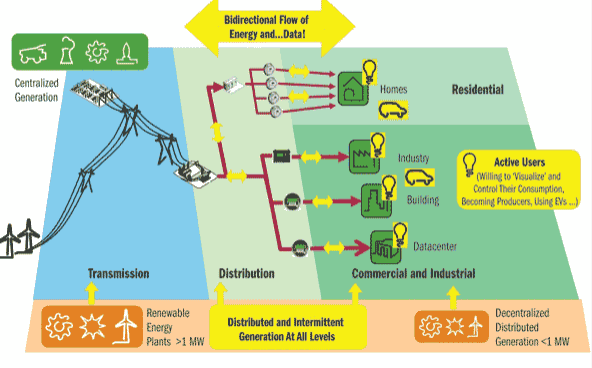
\includegraphics[width=0.9\textwidth]{img/teoria/sg.png}
  \caption{Flujo bidireccional de datos y energía en una \textit{smart grid} \cite{sins}}
  \label{fig:bidireccional}
\end{figure}

\vspace{3mm}

\begin{figure}[h!]
  \centering
  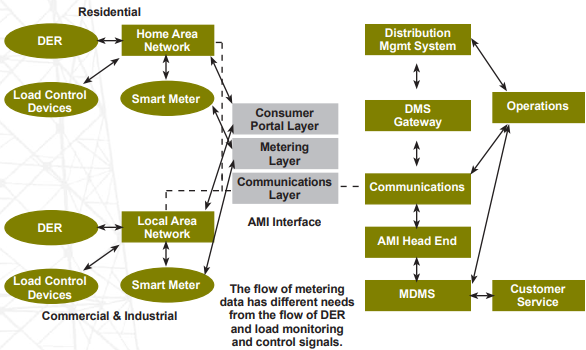
\includegraphics[width=0.9\textwidth]{img/teoria/bidir.png}
  \caption{Infraestructura de una interfaz \gls{ami} para el flujo bidireccional de energía y datos \cite{us}}
  \label{fig:bidireccional2}
\end{figure}

Es decir, en una red tradicional al ser unidireccional, se provee energía desde el distribuidor hacia el consumidor sin llevar a cabo ningún análisis estadístico sobre el consumo que se está produciendo en las líneas finales en un determinado instante temporal. En cambio, en el contexto de las \gls{sg}s, se pone el foco en las acciones de los usuarios y en la consecuente asignación de patrones de consumo eléctrico que permita predecir el comportamiento futuro de los mismos. \cite{convencional}

\vspace{3mm}

Sin embargo, como se expondrá más adelante en la Sección \ref{sec:consumo}, este proceso de clasificación de usuarios requerirá del análisis de grandes volúmenes de datos adquiridos a tiempo real, por lo que se aumentará la complejidad del sistema a costa de alcanzar la eficiencia.

\vspace{3mm}

Por lo tanto, teniendo en cuenta la característica de red bidireccional, se puede expresar que los propios usuarios son el gran pilar sobre el que se cimienta el sistema. En comparación a la red eléctrica tradicional, toman un papel mucho más activo monitorizando continuamente su comportamiento eléctrico y recopilando información para trasladarla al resto de la red. Esto tiene como ventaja una gran reducción de los costes derivados de la distribución y transmisión en el sistema, ya que se evita proporcionar más cantidad de energía de la requerida por las líneas finales. \cite{iotfutura}

\vspace{3mm}

Es por ello que se emplea una Infraestructura Avanzada de Medición (del inglés \gls{ami}) con una interfaz constituida por varias capas o niveles como se puede apreciar en la Figura \ref{fig:bidireccional2}. De esta forma, se dividen los flujos de comunicación entre las diferentes entidades que componen la red para permitir una mejor gestión de los mismos. \cite{us}

\vspace{1mm}

%%%%%%%%%%%%%%%%%%%%%%%%%%%%%%%%%%%%%%%%%%%%%%%%%%%%%%%%%%%%%%%%%%
\subsection{Prosumidores y microgrids}
\label{sec:prosu}

Dentro del presente contexto, en referencia a los usuarios es preciso introducir el término de prosumidor \cite{prosumer}. Se puede determinar como prosumidora a toda entidad o usuario final que tiene la capacidad de producir de forma alternativa recursos energéticos, además de poder consumirlos. En la Figura \ref{fig:prosumer} se puede visualizar cómo se estructura la \gls{sg} en un conjunto de distintas comunidades o agregaciones de prosumidores con el fin de crear microrredes de distribución y almacenamiento energético (del inglés \textit{microgrids}).

\begin{figure}[h!]
  \centering
  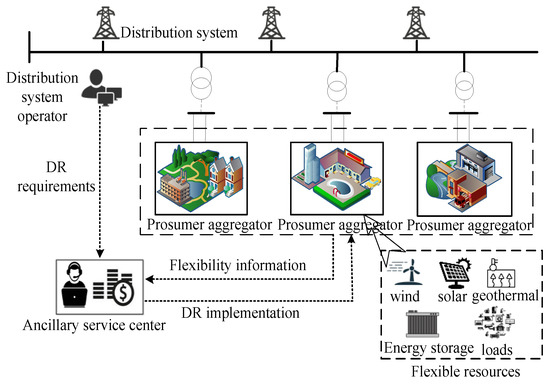
\includegraphics[width=1\textwidth]{img/teoria/prosumer.jpg}
  \caption{Estructura de la respuesta a la demanda en el contexto de una \textit{smart grid} con prosumidores \cite{prosumer}}
  \label{fig:prosumer}
\end{figure}

En este caso es imprescindible que los equipos y dispositivos dedicados a la generación de electricidad se encuentren dentro de la microrred o en una ubicación cercana a la misma. Así, se podrá abastecer a los usuarios del conjunto de forma eficiente, reduciendo los costes relacionados con la transmisión energética. 

\vspace{3mm}

Este tipo de esquema puede ser aplicado en diferentes entornos, como pueden ser los residenciales, industriales o agrícolas, para conseguir descentralizar la gestión de los recursos. Sin embargo, debe existir cierta gestión externa y coordinada de todas estas microrredes o comunidades de usuarios. Esta es llevada a cabo por una entidad denominada como operador del sistema distribuido (del ingles \gls{dso}) \cite{transactive} \cite{dso}. Algunas de sus funciones principales se basan en asegurar el abastecimiento de recursos en el interior de las microrredes en función de la demanda existente y en supervisar el estado operativo la infraestructura de red para garantizar su estabilidad y seguridad. 

\vspace{3mm}

Por otro lado, se encuentra también la figura del centro de servicios auxiliares \cite{transactive}, que se encarga de recibir la información sobre los recursos energéticos de los prosumidores y cuantificar en función de la oferta y demanda el beneficio económico que obtendrán los prosumidores. Estos normalmente son gestionados por los operadores del mercado eléctrico, pero puede variar según la región o el país.

\vspace{3mm}

\subsubsection{Mercado energético}

Las agregaciones de prosumidores posibilitan el autoconsumo y la compartición de los recursos generados por sí mismos con los demás participantes de la microrred, incluso con el resto de la \gls{sg}. La mayoría de los prosumidores, sobre todo en entornos residenciales son de pequeño tamaño y tienen mayores complicaciones para participar en los mercados eléctricos por sí mismos. 

\vspace{3mm}

Por ello, los agregadores \cite{bidding} \cite{transactive} se encargan de facilitar esta tarea para que una cantidad de prosumidores locales puedan actuar en conjunto como fijadores de precios de compra/venta en el mercado eléctrico global. Es decir, cada agregador se encarga de representar a los prosumidores que lo componen y actúa como intermediarios entre los mismos y el conjunto de mercados energéticos. 

\vspace{3mm}

A cambio, cada prosumidor debe pagar un plan mensual a la compañía para cubrir los costes eléctricos y así, dejar la responsabilidad de las transacciones a los agregadores para que operen de forma flexible. En esta operativa también incide el \gls{dso}, el cual se encarga de que las transacciones de compra/venta sigan el cumplimiento de los estándares y regulaciones establecidos en el mercado energético. 
\vspace{3mm}

\begin{figure}[h!]
  \centering
  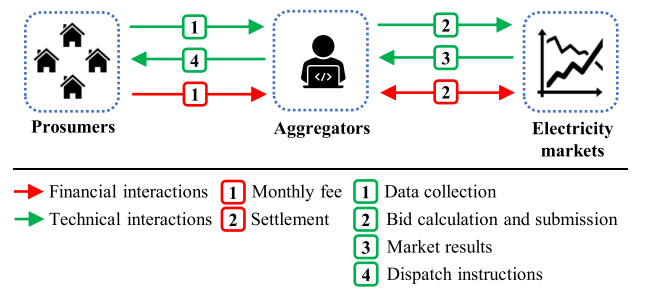
\includegraphics[width=0.9\textwidth]{img/teoria/market.png}
  \caption{Modelo basado en las interacciones de los agregadores con los prosumidores y el mercado eléctrico \cite{business}}
  \label{fig:market}
\end{figure}

\vspace{3mm}

A partir del funcionamiento expuesto y de la Figura \ref{fig:market}, se pueden diferenciar los tipos de interacciones que se producen en este modelo \cite{business}:

\begin{itemize}
  \item Interacciones técnicas 
    \begin{enumerate}
      \item Recopilación y adquisición de datos sobre los recursos de los prosumidores para su posterior procesamiento en los agregadores.  
      \item Cuantificación y presentación de ofertas desde los agregadores hacia los mercados mayoristas de electricidad.
      \item Comunicación de los resultados de diferentes mercados a los agregadores.
      \item Envío de instrucciones o recursos distribuidos en función de los resultados del mercado.      
    \end{enumerate}

  \item Interacciones financieras
  \begin{enumerate}
    \item Pago de tarifa mensual de cada prosumidor al agregador.
    \item Liquidación de las transacciones trasladadas desde los prosumidores en el mercado eléctrico (cobro por demanda y pago por generación).    
  \end{enumerate}
\end{itemize}

\vspace{1mm}

En cuanto al proceso de fijación de precios, generalmente, se adoptan tarifas minoristas dinámicas según el instante temporal, como pueden ser la fijación de precios por tiempo de uso (del inglés \gls{tou}) o en tiempo real (del inglés \gls{rtp}). Dentro de este contexto es preciso introducir los programas de gestión del lado de la demanda (del inglés \gls{dsm}). Como término, un programa \gls{dsm} es un programa basado en el control de las interacciones de consumo y de gestión de cargas residenciales desde el lado del cliente. 

\vspace{3mm}

Teniendo en cuenta el modelo de interacciones expuesto anteriormente, se puede expresar que un \gls{dsm} tiene como pilar fundamental la distribución de recursos energéticos de manera eficiente y acorde a la demanda y a la oferta. Permite reducir el coste de la adquisición energética y los costes asociados a la distribución como consecuencia de minimizar el número de interacciones necesarias entre el prosumidor y el resto de entidades del sistema. \cite{dsm}

\vspace{3mm}

Por lo tanto, volviendo a los modos de dinamización de las tarifas, si por ejemplo se emplea \gls{rtp}, se buscará lograr el equilibrio de la demanda en tiempo real, modificando las cargas de los consumidores en las horas pico \cite{rtp}. Es decir, cada uno de los usuarios actúa individualmente en función de los precios dinámicos en el tiempo, comunicándose directamente con la compañía energética como se puede visualizar en la Figura \ref{fig:dsm1}. 

\begin{figure}[h!]
  \centering
  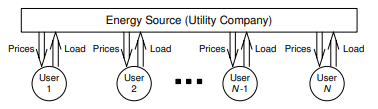
\includegraphics[width=0.8\textwidth]{img/teoria/dsm1.png}
  \caption{Estrategia de \gls{dsm} basada en interacciones individuales de cada consumidor con la compañía \cite{pricing}}
  \label{fig:dsm1}
\end{figure}

Con este proceso, el consumidor como puede saber en tiempo real la tarifa a la que está consumiendo energía, puede trasladar su propia carga desde las horas donde el precio es más alto (horas pico) a las de precio menor (horas valle). Esta gestión produce por tanto, menores picos de demanda y contribuyendo a la bajada de los precios. \cite{dsm} \cite{pricing}

\vspace{3mm}

No obstante, el diseño de un programa \gls{dsm} ideal en el contexto de las \gls{sg}s debería permitir también las interacciones entre los mismos prosumidores dentro de una zona residencial o microgrid. Estas interacciones generalmente se automatizan a través de equipos dedicados a una comunicación digital bidireccional. Como se aprecia en la Figura \ref{fig:dsm2}, este proceso tiene como fin conducir a una coordinación de las acciones respectivas a las cargas de un área determinada. 

\vspace{3mm}

Por tanto, en este caso la monitorización de las cargas totales para todos los nodos participantes en un instante determinado aportará la información necesaria sobre la relación entre la potencia pico y promedio (del inglés \gls{par}) y contribuirá a la fijación del precio unitario para ese mismo instante. \cite{pricing} 

\begin{figure}[h!]
  \centering
  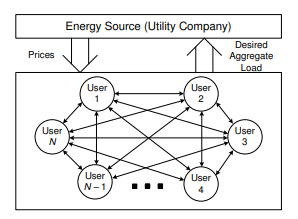
\includegraphics[width=0.65\textwidth]{img/teoria/dsm2.png}
  \caption{Estrategia de \gls{dsm} para smart grids basada en interacciones entre los usuarios y la compañía \cite{pricing}}
  \label{fig:dsm2}
\end{figure}


%%%%%%%%%%%%%%%%%%%%%%%%%%%%%%%%%%%%%%%%%%%%%%%%%%%%%%%%%%%%%%%%%%
\subsection{Estructura de una Smart Grid}

Una \gls{sg} está constituida por múltiples elementos diferentes como se puede visualizar en la Figura \ref{fig:estructura_sg}. Cada uno de ellos está dedicado a uno de los procesos principales, que se pueden dividir en generación, distribución y consumo. \cite{smartgrid_overview}

\begin{figure}[h!]
  \centering
  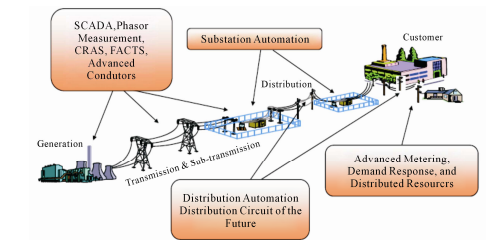
\includegraphics[width=1\textwidth]{img/teoria/estructura_sg.png}
  \caption{Estructura de componentes de una \gls{sg} \cite{smartgrid_overview}}
  \label{fig:estructura_sg}
\end{figure}

\subsubsection{Generación}

Como ya se introducía en la Sección \ref{sec:prosu}, dentro de una \gls{sg}, el prosumidor se trata de la figura que potencia principalmente el uso de energías renovables, las cuales pueden ser obtenidas por ejemplo a partir de generadores térmicos fotovoltaicos (del inglés \gls{pvt}) o de turbinas eólicas. Para posibilitar posteriormente el uso de la energía generada, esta debe ser convertida y acondicionada mediante dispositivos dedicados, como son unidades combinadas de calor (del inglés \gls{chp}) o de conversión a gas (del inglés \gls{p2g}). \cite{transactive}

\vspace{3mm}

Las unidades \gls{chp} \cite{chp} llevan a cabo un aprovechamiento del calor residual que deriva del proceso de generación de electricidad. Se emplean como respaldo eléctrico, ya que se componen de sistemas de almacenamiento de energía térmica (del inglés \gls{tes}) para poder separar la producción y el uso del calor y la energía. Luego, este calor almacenado se puede emplear en aplicaciones térmicas como la calefacción u otros procesos industriales. Es por ello que las unidades \gls{chp} mejoran la eficiencia del sistema energético, contribuyendo a un uso mucho más eficaz de los recursos y a una reducción de las pérdidas que se producen en la transmisión. En la Figura \ref{fig:chp} se representa a modo esquemático el funcionamiento de una unidad \gls{chp}. \cite{chp2}

\begin{figure}[h!]
  \centering
  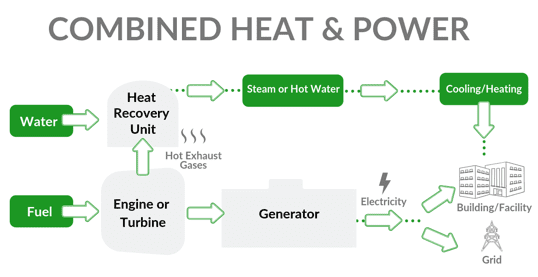
\includegraphics[width=0.9\textwidth]{img/teoria/chp.png}
  \caption{Esquema de funcionamiento de una unidad \gls{chp} \cite{chp}}
  \label{fig:chp}
\end{figure}

Además del \gls{tes}, utilizado para almacenar el calor producido, una unidad \gls{chp} también se constituye de un motor acoplado a un generador eléctrico para llevar a cabo el proceso de generación de electricidad y calor. Como se puede apreciar en la Figura \ref{fig:chp2}, todas las operaciones de la unidad y las interacciones que se producen entre módulos se coordinan desde el gestor de operaciones para que se produzca un correcto funcionamiento.

\begin{figure}[h!]
  \centering
  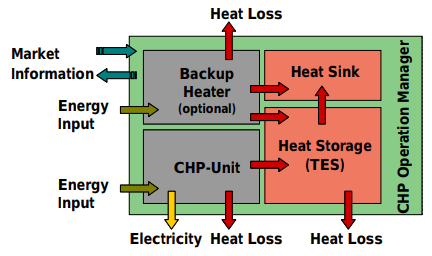
\includegraphics[width=0.65\textwidth]{img/teoria/chp2.png}
  \caption{Gestión de operaciones en una unidad \gls{chp} \cite{chp2}}
  \label{fig:chp2}
\end{figure}

Por otro lado, la unidad \gls{p2g}, mencionada anteriormente, se encarga de la conversión de la electricidad en gases sintéticos, como son el hidrógeno o el metano. Es de gran importancia, ya que este tipo de gases son más fácil de transportar y almacenar que la electricidad, por lo que se simplifica la gestión energética. \cite{transactive}

\vspace{3mm}

Como se puede apreciar en la Figura \ref{fig:p2g}, el objetivo del \gls{p2g} se basa en descomponer el agua mediante un proceso de electrólisis a partir de electricidad proveniente de fuentes renovables. Después, el hidrógeno que se produce se puede utilizar directamente o procesarlo de forma adicional en metano. 

\begin{figure}[h!]
  \centering
  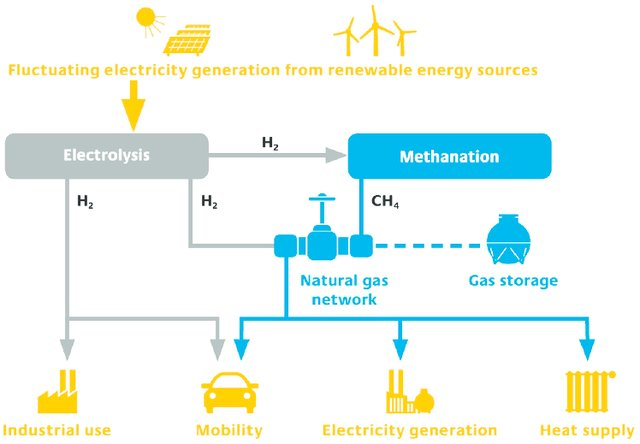
\includegraphics[width=0.85\textwidth]{img/teoria/p2g.jpg}
  \caption{Representación del proceso \gls{p2g} \cite{p2g}}
  \label{fig:p2g}
\end{figure}

Dentro del contexto de la generación de energía también es importante destacar algunos equipos, como son los sistemas de control y adquisición de datos (del inglés \gls{scada}) \cite{scada}. Estos pueden ser instalados en generadores, como son paneles solares fotovoltaicos o turbinas eólicas, consiguiendo una monitorización remota de los mismos. Mediante la información recopilada a tiempo real permiten conocer los niveles de generación y establecer una predicción de la disponibilidad energética que habrá en el sistema o en un área determinada del mismo.

\vspace{3mm}

\subsubsection{Distribución}

Un dispositivo importante en el campo de la distribución energética es la Unidad de Medición de Fasores (del inglés \gls{pmu}). Se emplea para medir con una alta precisión los fasores de tensión y corriente en la red eléctrica, proporcionando información relevante sobre las magnitudes y fases de las ondas sinusoidales. 

\vspace{3mm}

También, es empleado en los generadores y debe contar con una alta tasa de muestreo para capturar eventos transitorios o cambios rápidos en la red. En otros términos, debe tener la capacidad de identificar o detectar a tiempo real posibles anomalías que se puedan dar en la distribución y por ello, se trata de un componente imprescindible para comprobar y garantizar la estabilidad de la \gls{sg}. %BIB

\vspace{3mm}

La confiabilidad y la seguridad de la red también reside en los Sistemas de Transmisión de Corriente Alterna Flexibles (del inglés \gls{facts}) \cite{facts} \cite{facts3}. Estos vienen dados por la necesidad de superar las limitaciones técnicas introducidas por las redes eléctricas, como son las térmicas o las respectivas al voltaje. En otros términos, incrementan la potencia transmitida y aportan flexibilidad al permitir modificar de forma dinámica los parámetros eléctricos ante cambios en la configuración de la red. 

\vspace{3mm}

Los \gls{facts} incluyen todos los elementos electrónicos basados en tecnología de alta potencia y que son empleados dentro de una \gls{sg} para la transferencia de energía de CA y el control de la potencia reactiva. También, realizan tareas de reducción de impedancia en las líneas de transmisión y de optimización del factor de potencia y pueden actuar tanto a nivel individual como de forma coordinada con otros controladores.

\vspace{3mm}

La primera generación de \gls{facts} emplea interruptores controlados por tiristores, mientras que la segunda tiene como base convertidores estáticos de conmutación. En la Tabla \ref{tab:facts} se visualizan las tecnologías \gls{facts} más relevantes. \cite{facts2} \cite{facts3}

\begin{table}[!h]
    \centering
    \resizebox{\textwidth}{!}{
    \begin{tabular}{| c | c | m{6cm} |}
    \hline
    \rowcolor[HTML]{EFEFEF}
    Generación & Tipo & \multicolumn{1}{c|}{Descripción} \\ \hline
    \multirow{2}{*}{1º} 

    & \gls{tcsc} & Controla el flujo de potencia tanto reactiva como activa por la línea de transmisión mediante el ajuste de impedancia en serie y amortigua las oscilaciones.
    
    \\ \cline{2-3}

    & \gls{svc} & Absorbe o suministra potencia reactiva según las necesidades de una línea de transmisión a través de la variación de la susceptancia en paralelo. Ayuda a mantener el voltaje estable en la red y proveen un aumento de la capacidad de transferencia de energía.

    \\ \hline
    \multirow{4}{*}{2º} 
    
    & \gls{statcom} & Compensa la potencia reactiva al igual que el \gls{svc}, pero en este caso empleando electrónica de potencia para proporcionar una respuesta más rápida.

    \\ \cline{2-3} 

    & \gls{upfc} & Combina las funciones de un \gls{tcsc} y un \gls{svc}, teniendo la capacidad de controlar en una línea de transmisión tanto la impedancia en serie como la susceptancia en paralelo.

    \\ \cline{2-3} 

    & \gls{sssc} & Modifica dinámicamente la impedancia y es capaz de controlar la fase y la amplitud de la tensión en la línea.

    \\ \cline{2-3} 

    & \gls{ipfc} & Conecta varias líneas de transmisión en paralelo. No obstante, modula la impedancia y la fase de la tensión de cada línea de transmisión de forma independiente, lo que permite operar sobre el flujo de potencia de una forma controlada. Mejora la capacidad de transmisión y reduce las pérdidas energéticas. 
    
    \\ \hline
    \end{tabular}
    }
    \caption{Tecnologías FACTS de 1ª y 2ª generación}
    \label{tab:facts}
\end{table}

Poniendo el enfoque en la garantía de estabilidad de una \gls{sg}, uno de los sistemas más importantes de los expuestos en la Tabla \ref{tab:facts} es el \gls{svc} \cite{facts}. Los compensadores estáticos son capaces de detectar grandes caídas de tensión resultantes a la producción de un cortocircuito o a la pérdida de líneas de transisión en un área de la red. Esto es importante, ya que una detección rápida de una avería permite restaurar en un corto período de tiempo la tensión del área afectada sin que el problema escale a otras partes de la red. 

\vspace{3mm}

En otros términos, aísla este área del resto de la red eléctrica. Además, el \gls{svc} asegura que el proceso de restauración se produzca paulatinamente para que los efectos producidos por el cortocircuito sean prácticamente imperceptibles en los puntos de carga del área afectada. En la Figura \ref{fig:svc} se puede apreciar un ejemplo de instalación de un \gls{svc} en el municipio noruego Sylling y se encuentra conectada a un sistema de 420 kV.

\begin{figure}[h!]
  \centering
  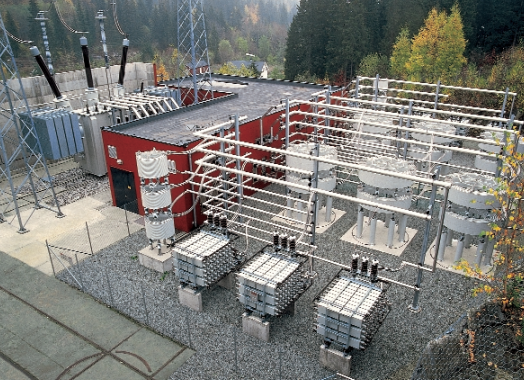
\includegraphics[width=0.7\textwidth]{img/teoria/svc.png}
  \caption{Instalación de un \gls{svc} en Sylling (Noruega) \cite{facts}}
  \label{fig:svc}
\end{figure}

Siguiendo en el ámbito de la distribución energética, es importante también exponer las tecnologías enfocadas a la transmisión de electricidad a larga distancia, como son las Corriente Continua de Alto Voltaje (del ingles \gls{hvdc}) \cite{hvdc}. Como su nombre indica, utilizan corriente continua para ello, lo que minimiza las pérdidas en el proceso de transmisión respecto al caso de la Corriente Alterna de Alto Voltaje (del ingles \gls{hvac}), además de permitir portar mucha más potencia. 

\vspace{3mm}

Esto es fundamental cuando se pretende integrar al sistema global fuentes de energía ubicadas en áreas remotas, sobre todo dentro del contexto de las \gls{sg}s. Generalmente, las fuentes de energías renovables, como pueden ser la solar o la eólica, se encuentran alejadas de los puntos geográficos con mayor demanda y se requiere una respuesta rápida ante cambios de carga para mantener la estabilidad del sistema. 

\vspace{3mm}

Es decir, cuando se transmiten grandes cantidades de potencia a largas distancias con líneas de \gls{hvac}, se generan ángulos eléctricos entre los voltajes y las corrientes en la línea muy grandes que pueden producir oscilaciones descontroladas y por tanto, desencadenar inestabilidades que llegaráin a escalar a lo largo del sistema. 

\vspace{3mm}

Por ello, las tecnologías \gls{hvdc} simplifican la interconexión entre microrredes y permiten una mayor integración de sistemas dedicados al almacenamiento energético para facilitar la gestión de los recursos disponibles. Como desventaja, se encuentra el alto coste que supone su implementación, ya que al final solamente se puede emplear en el caso de aplicaciones punto a punto.

\vspace{3mm}

En la Figura \ref{fig:hvdc} se muestra como ejemplo una infraestructura de transmisión de energía eólica a larga distancia. Esta energía proviene de una fuente remota y se transporta a través del medio marino para llegar hasta los usuarios. Como se puede apreciar, es necesario implementar estaciones de conversión de alto voltaje de corriente alterna a continua y viceversa en los extremos de las líneas \gls{hvdc}.

\begin{figure}[h!]
  \centering
  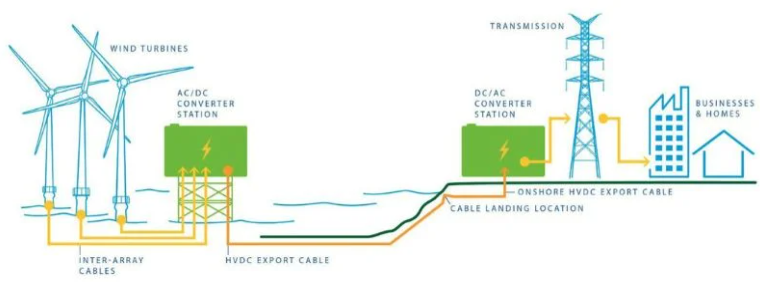
\includegraphics[width=0.9\textwidth]{img/teoria/hvdc.png}
  \caption{Representación de un sistema de transmisión de energía eólica con líneas \gls{hvdc} \cite{hvdc2}}
  \label{fig:hvdc}
\end{figure}

\subsubsection{Consumo}
\label{sec:consumo}

Entrando en detalle en las ubicaciones finales del sistema y por tanto, en el proceso de consumo, es imprescindible conocer la cantidad de energía demandada por los clientes que pertenecen a una \gls{sg}. La instalación de sensores o medidores inteligentes (del ingles \textit{smart meters}) en las viviendas posibilitan el registro constante de datos respectivos al consumo de energía, niveles de voltaje, corriente y factor de potencia. Estos son almacenados, analizados y procesados por las distribuidoras de energía para obtener a partir de los mismos la información necesaria sobre el comportamiento de los usuarios. \cite{stab}

\vspace{3mm}

Como se había introducido en el Apartado \ref{sec:smartgrids} el proceso de adquisición de datos por parte de los usuarios se trata de uno de los pilares más relevantes de cara a la optimización energética del sistema. Los objetivos principales que se pretenden con este proceso se engloban en la reducción del consumo, la optimización de la distribución y la maximización del beneficio. Respecto a este último, las compañías energéticas a partir de su base de clientes estudian las estrategias de categorización de los mismos para definir el sistema de fijación de precios dinámicos. \cite{stab}

\vspace{3mm}

No obstante, la gestión de los sensores finales en las \gls{sg}s se caracteriza por su alta complejidad, debido a los grandes volúmenes de datos a manejar. Se requiere un procesamiento eficiente a tiempo real para analizar datos capturados de múltiples fuentes con el fin de evitar latencias o bloqueos en el sistema. Es por ello que se dificulta el empleo de herramientas convencionales de gestión de bases de datos y se requiere una solución más avanzada mediante la aplicación de tecnologías enfocadas al \textit{Big Data}. Se profundizará más sobre ello en la Sección \ref{sec:bigdata}.

\vspace{1mm}

%%%%%%%%%%%%%%%%%%%%%%%%%%%%%%%%%%%%%%%%%%%%%%%%%%%%%%%%%%%%%%%%%%
\subsection{Protocolos}
% a) Green-RPL
% (b) Local positive degree coupling
% (c) IEEE 802.11s
% (d) Web Of Energy
% (e) Dynamic Barrier Coverage
% (f) IEC61850
% (g) Wind-driven bacterian foraging algorithm
% (h) Data Slicing
% (i) TSUBE energy trading algorithm
% (j) Stochastic Geometry
% (k) Rectangular quadrature amplitude modulation
% (l) Policy-based group authentication algorithm
% (m) Mapping interface integration COIIoT
% (n) Nash Equilibrium (NE) and the Bayesian NE
% (o) Wireless sensor network protocol
% (p) Algorithmic Approach


%Green-RPL, Local positive degree coupling, IEEE 802.11s, Web Of Energy, Dynamic Barrier Coverage, IEC61850, Wind-driven bacterial foraging algorithm, Data Slicing, TSUBE energy trading algorithm, Stochastic Geometry, Rectangular quadrature amplitude modulation, Policy-based group authentication algorithm, Mapping interface integration COIIoT, Nash Equilibrium (NE) and the Bayesian NE, Wireless sensor network protocol and Algorithmic Approac

%ver tabla https://electrical-engineering-portal.com/smart-grid-deployment-what-weve-done-so-far


\vspace{1mm}

%%%%%%%%%%%%%%%%%%%%%%%%%%%%%%%%%%%%%%%%%%%%%%%%%%%%%%%%%%%%%%%%%%
\subsection{Topología de red}

% Smart Grid Network Topology
% (a) Neighborhood Area Networks (NAN)
% (b) Software-Defined Networks (SDN)
% (c) Interdependent Networks (IN)
% (d) Field Area Networks (FAN)
% (e) Wireless Sensor Networks (WSN)
% (f) Not Defined
%NAN, FAN AND THE SDN are widely used network topology



\vspace{1mm}

%%%%%%%%%%%%%%%%%%%%%%%%%%%%%%%%%%%%%%%%%%%%%%%%%%%%%%%%%%%%%%%%%%
\subsection{Seguridad en Smart grids}
\label{sec:seg}
 
Como se ha introducido en la Sección referente a la figura del prosumidor (ver Sección \ref{sec:prosu}), el \gls{dso} tiene la capacidad de operar ante problemas y fallos en la red tomando decisiones y dando una respuesta rápida. En determinados casos las incidencias se pueden dar por la configuración del propio sistema, si esta no se realiza de forma correcta y eficiente. No obstante, también es preciso contemplar la posibilidad de ataques externos que atenten contra el sistema de la \gls{sg}.

\vspace{3mm}

Uno de los ataques más peligrosos en este ámbito es el de Inyección de Datos Falsos (del inglés \gls{fdi}) \cite{baddata} y, como su nombre determina, se basa en la inyección de paquetes maliciosos en la red con el fin de bloquear los servicios de la misma y conseguir la autorización para realizar operaciones restringidas. El proceso se puede realizar actuando directamente a través de los sensores finales (\textit{smart meters}) o secuestrando el canal de comunicación. Algunas técnicas empleadas por los atacantes son las siguientes \cite{baddata}:

\begin{itemize}
  \item Fallo del dispositivo: Se aplica un ataque de Denegación de Servicio (del inglés \gls{ddos}) a los sensores. Cabe destacar que generalmente los sensores que se encuentran en las ubicaciones finales tienen una capacidad limitada de conexión que derivaría en grandes latencias en la comunicación de datos con el resto de entidades de la red. En este momento el atacante se encarga de suplantar al host en cuestión para enviar los paquetes falsos en su nombre.
  \item \textit{Cracking}: Se descifran las contraseñas para obtener acceso a los equipos mediante ingeniería social o fuerza bruta. De la misma forma que el anterior, la limitación de los recursos computacionales de los sensores provoca que no existan mecanismos de contraseñas lo suficientemente seguros. Además, la mayoría de ellos emplean como protocolos de comunicación Modbus/TCP o DNP 3.0/TCP, los cuales implementan una transmisión de texto en formato plano y sin cifrado. Por ello, un atacante puede tener la posibilidad de monitorear y capturar el tráfico si consigue acceso.
  \item Envenenamiento de tablas \gls{arp} o \textit{\gls{arp} Spoofing} \cite{arp}: Consiste en enviar mensajes falsos \gls{arp} para monitorizar el tráfico y capturar o alterar los paquetes que se están transmitiendo por la red. 
\end{itemize}

Teniendo esto en cuenta, es imprescindible definir los mecanismos de detección y mitigación a emplear para evitar que se produzcan ataques \gls{fdi} \cite{baddata}:

\begin{itemize}
  \item Mecanismo de autenticación estrictos: Los datos que se suministran al \gls{dso} o a otras entidades de control de la \gls{sg} deben de ser autenticados para comprobar su confiabilidad. Para ello, se emplean por ejemplo, marcas de tiempo para evitar ataques de repetición y protocolos de seguridad como \gls{tls} o \gls{ssl}, además de \gls{sha} y \gls{hmac}.
  \item Gestión dinámica de claves: Se actualizan las claves con una determinada frecuencia para incrementar la seguridad de los estándares \gls{ieee} 802.11s y evitar ataques \gls{ddos}.
  \item Empleo del protocolo \gls{send} \cite{send}: Para evitar los ataques de \textit{\gls{arp} Spoofing} se emplean pares de claves \gls{rsa} para poder garantizar en el proceso de enrutamiento que los mensajes que tienen como origen un determinado host pertenecen al mismo.
\end{itemize}



%a partir del 3.4 del AI-based FDI Countermeasure for IoE Smart Grids

%%%Energy Big Data: A Survey pag 10 figura















\vspace{1mm}

%%%%%%%%%%%%%%%%%%%%%%%%%%%%%%%%%%%%%%%%%%%%%%%%%%%%%%%%%%%%%%%%%%
\subsection{Estándares y regulación en smart grids}

%estándares smart grids -> cite OUTLOOK FOR INCREASED ADOPTION OF SMART GRID TECHNOLOGIES IN ADB ENERGY SECTOR OPERATIONS

% International Technical Standards for Smart Grids (Smart Grid Codes)
% Grid code development and implementation is a critical area in smart grid implementation. It has to be 
% aligned with the standards being used in respective countries and international standards. This is an 
% important first step in smart grid implementation. Some of the international standards are as follows.
% (i) IEEE1547 Family of Standards. IEEE 1547 family of standards deals with smart grid components 
% involving distributed resources interconnection. Released in 2003, this provides the basis and 
% sets the standards for the integration of distributed energy generation by detailing requirements 
% related to interconnection performance, operation, testing, safety, and maintenance.
% (ii) IEEE 2030 Family of Standards. The  IEEE Standard 2030–2011’s “Guide for Smart Grid 
% Interoperability of Energy Technology and Information Technology Operation with the 
% Electric Power System, and End-Use Applications and Loads” is the root standard of the 2030 
% series. This standard provides alternative approaches and best practices for achieving smart 
% grid interoperability.
% (iii) IEC Family of Standards. IEC has identified over 100 standards relevant to smart grids. The 
% following are core standards: (i) IEC/TR 62357: Service Oriented Architecture; (ii) IEC/61970: 
% Common Information Model/Energy Management; (iii) IEC 61850: Power Utility Automation; 
% (iv) ICC/61968: Common Information Model/Distribution Management; IEC 62351: Security; 
% (v) IEC 62056: Data Exchange for Meter Reading, Tariff and Load Control; and (vi) IEC 61508: 
% Functional Safety of Electrical, Electronic, Programmable Electronic Safety Related Systems.


\vspace{1mm}

%%%%%%%%%%%%%%%%%%%%%%%%%%%%%%%%%%%%%%%%%%%%%%%%%%%%%%%%%%%%%%%%%%
\subsection{Beneficios ambientales}

%Las smart grid son un concepto estratégico clave en la transición energética, ya que suponen un gran paso hacia un mundo descarbonizado. Mediante la digitalización de las redes eléctricas inteligentes se puede conseguir un sistema más eficiente, sostenible, con bajas pérdidas y con altos niveles de calidad en el suministro. Con la implementación de este circuito inteligente no solo se conseguiría una mayor eficiencia energética y ahorro, sino que también tendría múltiples beneficios medioambientales, económicos y sociales.


% La eficiencia energética que se pueden conseguir con las smart grid también tiene beneficios directos sobre el medio ambiente, como por ejemplo: 

% Permiten el desarrollo de ciudades sostenibles.
% Pueden integrarse en el sistema de fuentes renovables.
% Facilitan la movilidad eléctrica, proporcionando puntos de carga para vehículos eléctricos.
% Reducen las emisiones globales de CO2.
% Contribuye a la descarbonización de la generación eléctrica. 


\vspace{1mm}

%%%%%%%%%%%%%%%%%%%%%%%%%%%%%%%%%%%%%%%%%%%%%%%%%%%%%%%%%%%%%%%%%%
\subsection{Situación en España}

En el caso de España, nuestro país ocupa el quinto lugar en el mercado eléctrico europeo, solamente por detrás de Alemania, Francia, Reino Unido e Italia. 

%buscar datos españa

Además, en los último años ha crecido en consideración 

y está creciendo rápidamente. La demanda eléctrica estimada para el año 2001 fue de 210.4 mil millones de kilovatios-hora (bkwh), un aumento del 5% respecto al año 2000. Se estima que la demanda eléctrica de España aumentará un 30% para el año 2010.

% Para hacer frente al aumento de la demanda eléctrica en España, las empresas de servicios públicos nacionales han invertido en capacidad de generación y distribución. Red Eléctrica de España (REE), por ejemplo, invirtió considerablemente en la red en 2001, destinando 78.4 millones de euros a la expansión de la red eléctrica. En octubre de 2001, REE también anunció planes para invertir entre 60.2 y 72.2 millones de euros para mejorar la conexión eléctrica con Francia. Las tres mayores compañías eléctricas de España: Endesa, Iberdrola y Unión Fenosa, han dedicado 34 mil millones de euros en inversiones desde agosto de 2001 hasta 2005, gran parte de ellas en América Latina y otros países europeos, pero incluyendo aún así 8 mil millones de euros para nuevas plantas generadoras en España.

% Endesa está construyendo actualmente una planta de turbina de gas de ciclo combinado (CCGT) de 400 MW en Huelva, además de otras dos CCGT de gas de 400 MW que la empresa ya tiene en construcción en Barcelona y Tarragona. Endesa completó recientemente la construcción de una planta con 8,000 MW en Cádiz. Unión Fenosa planea agregar 5,000 MW de nueva capacidad para 2005, principalmente en España, de los cuales 2,800 MW serían de gas natural. Piemsa, una filial de Petronor, planea construir un complejo de gasificación integrada de ciclo combinado (IGCC) de 800 MW en una refinería cerca de Bilbao que utilizará productos pesados de la refinería. La planta será una de las más grandes y avanzadas de su tipo en el mundo.


%https://www.smartgridsinfo.es/2020/01/23/6-congreso-smart-grids-refuerza-consolida-redes-electricas-inteligentes-politica-energetica-espana

\cite{spain}


\begin{figure}[h!]
  \centering
  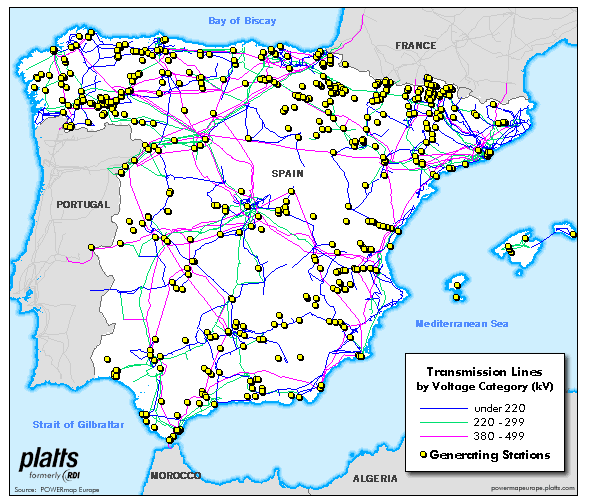
\includegraphics[width=0.8\textwidth]{img/teoria/spain.png}
  \caption{Red nacional de transmisión energética \cite{spain}}
  \label{fig:spain}
\end{figure}







\vspace{1mm}

%%%%%%%%%%%%%%%%%%%%%%%%%%%%%%%%%%%%%%%%%%%%%%%%%%%%%%%%%%%%%%%%%%
\subsection{Desafíos futuros de las smart grids}

%%%%\cite{overview} Smart Grid: An Overview

% The Key Challenges for Smart Grids 
%  Strengthening the grid—ensuring that there is sufficient transmission capacity to interconnect energy resources, especially renewable resources; 
%  Moving offshore—developing the most efficient connections for offshore wind farms and for other marine 
% technologies; 
%  Developing decentralized architectures—enabling smalller scale electricity supply systems to operate harmoniously with the total system; 
%  Communications—delivering the communications infrastructure to allow potentially millions of parties to 
% operate and trade in the single market; 
%  Active demand side—enabling all consumers, with or 
% without their own generation, to play an active role in 
% the operation of the system; 
%  Integrating intermittent generation—finding the best 
% ways of integrating intermittent generation including 
% residential microgeneration; 
%  Enhanced intelligence of generation, demand and most 
% notably in the grid; 
%  Preparing for electric vehicles—whereas Smart Grids 
% must accommodate the needs of all consumers, electric vehicles are particularly emphasized due to their 
% mobile and highly dispersed character and possible 
% massive deployment in the next years, what would 
% yield a major challenge for the future electricity networks [2]. 




%%%%cite us


%4.0 Desafíos para la implementación
% Entre los desafíos importantes que enfrenta el desarrollo de una red inteligente se encuentran el costo de
% de implementación de una red inteligente, con estimaciones solo para la medición avanzada de la empresa eléctrica
% de capacidad que asciende a $27 mil millones, y las regulaciones que permiten la recuperación de dicha
% inversiones. Para tener una perspectiva, Brattle Group estima que podría tomar tanto como
% 1,5 billones de dólares para actualizar la red para 2030 (Chupka et al. 2008). Garantizar la interoperabilidad % de estándares de redes inteligentes es otro obstáculo que los reguladores estatales y federales deberán superar.
% Las principales barreras técnicas incluyen el desarrollo de sistemas de almacenamiento económicos; estos sistemas de almacenamiento
% puede ayudar a resolver otros desafíos técnicos, como la integración de energía renovable distribuida
% de fuentes con la red, abordando problemas de calidad de energía que de otro modo exacerbarían la
% de situación y mejorar la utilización de los activos. Sin red inteligente, altas penetraciones de variables
% de recursos renovables (por ejemplo, eólicos o solares) pueden volverse cada vez más difíciles y costosos de obtener.
% logran con el tiempo a medida que penetran a niveles altos debido a la mayor necesidad de coordinar estos
% de recursos con generación despachable (p. ej., ciclo combinado de gas natural) y demanda.
% Otro desafío al que se enfrenta una red inteligente es la incertidumbre sobre el camino que seguirá su desarrollo.
% se hace cargo del tiempo con la tecnología cambiante, los cambios en las combinaciones de energía y la política energética.
% Intentar legislar o regular el desarrollo de una red inteligente o sus tecnologías relacionadas puede
% disminuyen gravemente los beneficios del mercado energético virtual, flexible y transparente al que se esfuerza.
% Para proveer. Por el contrario, con la red energética de todo el país potencialmente en riesgo, algunos pueden ver
% la introducción de una red inteligente en los Estados Unidos es demasiado importante para permitir el laissez-faire
% evolución. Por lo tanto, el desafío del desarrollo se convierte en una cuestión de proporcionar servicios flexibles
% de regulación que aprovecha la tecnología deseada y en desarrollo a través de objetivos dirigidos y
% de políticas respaldadas por casos de negocios que promueven un resultado económico positivo. Estos y otros
% de desafíos se analiza en las siguientes secciones


\subsubsection{Retos técnicos}

% There are a variety of technical challenges facing a smart grid, some of the greatest being 
% developing, implementing, and deploying the array of different technologies required to 
% enable both sides of the meter to communicate in a cost-effective way. One of the most 
% important developments facing a smart grid is AMI technology. These devices help 
% coordinate consumer equipment, as well as receive market signals and adjust household 
% consumption based on a combination of this data and consumer preferences. However, 
% alternatives to such AMI systems do exist. For example, market information such as prices 
% and grid conditions can be decoupled from communication of energy consumption. Thus, 
% the meter can be separate while pricing signals and the like can be transmitted via other public 
% communication mechanisms such as phone, internet, cable, and wireless radio. A decoupled 
% situation can make sense for commercial buildings and industrial uses where energy savings 
% can be significant, while a more traditional bundled AMI package may be more desirable for 
% residential consumers due to its “all-in-one” and “plug-and-play” aspects. Implementing 
% price- and consumption-bundled AMI technology has been estimated to cost as much as 
% $27 billion (Kuhn 2008) and will require very aggressive deployment to meet desired market 
% penetration levels in the near future. Failure to successfully deploy technology that captures 
% bi-directional power flow rather than net consumed energy, as well as dynamic pricing 
% support, such as AMI technology or others, will keep the two sides of the market from 
% properly communicating, and a smart grid will not function as desired regardless of other
% successful technical deployments, such as distributed generation, demand-response measures, 
% or automated distribution schemes. Without real-time demand-response signals being 
% promptly communicated and quickly addressed by consumers, the power system will not 
% be flexible enough to provide the market transparency or the price signals required for a 
% functioning energy market (FERC 2006a). Further, AMI billing techniques and the machines 
% themselves may require regional customization reducing potential economies of scale in 
% production and deployment. Regional customization may be required because of differences 
% in consumer preferences, aggressiveness of service providers, state and local regulations, and 
% the speed with which smart grid structures and technology change over time. Not all regions 
% are likely to respond identically and may have different needs.
% Another significant technical consideration is the impact of high levels of new technology 
% penetration on existing grid infrastructure. Implementing new improvements into the grid, 
% including smart-grid technologies, is pivotal to increasing efficient operations, as the operating 
% efficiency gains from familiar technologies have begun to plateau (DOE/EIA 2007a). In 
% addition, a NERC survey recently ranked the number one challenge to grid reliability as 
% “aging infrastructure and limited new construction.” How this aging infrastructure will 
% function when combined with new “smart” technology remains to be seen, particularly with 
% regard to solar, wind, and other forms of distributed generation (NERC 2007). Adding large 
% amounts of variable and distributed generation, for example, requires a fundamental 
% reworking of how the delivery system is managed, power quality is monitored, faults are 
% detected, and maintenance is handled (Pai 2002). This problem is compounded when 
% PHEVs and EVs are considered, potentially making each vehicle its own DG resource and 
% requiring supporting infrastructure to draw, generate, and price power transactions. 
% However, these technologies themselves face several technical challenges. Cost-effective 
% battery technology continues to be a challenge for PHEVs and EVs and local wind and solar 
% resources. Issues such as discharge, battery life, size and weight are all serious considerations. 
% Additionally, incorporating battery power storage into current automobile frames will require 
% manufacturing adjustments; including systems to monitor the status of the battery (including 
% battery charge and temperature) as well as structural design changes to accommodate the 
% battery itself.

% A smart grid is needed at the distribution level to manage voltage levels, reactive power, 
% potential reverse power flows, and power conditioning, all critical to running grid-connected 
% DG systems, particularly with high penetrations of solar and wind power and PHEVs. 
% Advanced voltage regulation, fault-detection, and system-protection practices need to be 
% rethought as an increasing number of DG resources become available. This may require new 
% equipment to identify and isolate DG resources in the event of a fault occurrence (Driesen 
% and Belmans 2006). Another consideration for power-generation systems, distributed or 
% otherwise, is power quality. Customers and the utilities that serve them lack standards for 
% classifying varying qualities of power. Because customers have different power quality 
% requirements (e.g., willingness to accept outages of varying durations, and load sensitivity to 
% power harmonics) and with the increasing availability of DG resources to produce power 
% locally, there may be smaller sub-markets for power that would be better served if such 
% differentiated power standards existed.
% Designing and retrofitting household appliances, such as washers, dryers, and water heaters 
% with technology to communicate and respond to market signals and user preferences via 
% home automation technology will be a significant challenge. Substantial investment will be 
% required to implement user-friendly communication equipment which ensures that data
% storage and transmissions are tamper proof, reliable, and do not corrupt or break down over 
% the lifetime of an appliance. Devices that communicate wirelessly with their facility energymanagement systems must broadcast powerful-enough signals, or other technical barriers to 
% effective communication must be resolved. For example, a washer/dryer located in a house’s 
% basement attempting to communicate with an energy-management system on the far side of 
% the building will require a stronger signal than a closer device on the ground floor. Therefore 
% communication equipment may need a flexible and dynamic range of broadcast strengths. 
% Finally, aggregating and sharing system data involves its own concerns; for example, providing 
% infrastructure to communicate wide-area measurement data across the grid requires agreement 
% by the stakeholders on the information network architecture, the supported functions, data 
% exchange interface definitions, and legal conditions for granting use of the data.

\subsubsection{Retos económicos}

% The business case for a smart grid needs to be firmly established for deployment decisions to 
% progress. In many situations, individual applications may not be cost effective in isolation, 
% but where common hardware and information network infrastructure can be leveraged to 
% accomplish a number of objectives, the value proposition can become compelling. The 
% business challenge is to prove that out with field deployments. Smart grid investments often 
% require large upfront costs relative to their benefits. However, future benefits may come at 
% small incremental costs. Utilities and regulators may need to look at full system life cycle 
% costs and benefits in order to fully justify added investments. Some of the benefits may come 
% in the form of societal benefits which will need to be clearly understood and evaluated. 
% Payback periods may be longer than stakeholders would like. The service providers, regulators, 
% and ultimately ratepayers are going to have to believe it before such substantial investments 
% are made.
% Since the technology and value propositions are emerging, utility companies may be reluctant 
% to expend the significant amount of capital required to move toward a smart grid, especially 
% because expected cost-recovery timelines are only theoretical and have no precedent. 
% Currently, regulated utilities and their flat-rate customers have no risk or reward signal. 
% Regulation makes it difficult for them to raise rates and recover costs, and makes them 
% reluctant to change. Moreover, transmission-planning difficulties may or may not offset 
% revenue losses incurred from reduced transmission; with uncertainty about market penetration 
% of DG these effects can be difficult to model. Without effective cost recovery mechanisms in 
% place, increased market penetration of DG will translate into lost demand for utilities. The 
% uncertainty about market penetration is increased when utilities start to consider the time and 
% cost of training a new smart-grid-skilled labor force (NERC 2007). Thus, utilities seeking to 
% balance costs and operating efficiency will seek to increase asset utilization through the 
% implementation of demand response measures and AMI technology, as opposed to expensive 
% infrastructure upgrades. Further, as more and more devices become “web enabled” and move 
% toward becoming fully “smart” devices, the inclusion of electronics in these devices, as well as 
% the development and maintenance of this hardware and its respective software, will require 
% manufacturers to reevaluate these devices’ life-cycle costs. A smart grid will require service 
% providers to operate in new ways and be willing to take reasonable risks for reasonable 
% rewards. Regulators will need to design rules such that customers who do not change are not 
% worse off, but that businesses can pursue advantageous arrangements between participating 
% suppliers and consumers. Aside from making a strong analytical business case with existing distribution models, the first 
% few successful deployments of these new “smart” technologies will be pivotal to ensuring deep 
% market penetration. Not all of these technologies are necessarily complementary. For 
% example, when metering residential customers, drive-by and walk-by meters (AMR) are 
% considered a competing technology and currently are out-shipping AMI products. Other 
% than the more-convenient data gathering over traditional meters, AMR meters offer very few 
% to none of the benefits and functions necessary to enable residential customers to 
% meaningfully participate in a smart grid. However, implementing smart-grid technologies is 
% daunting; the cost to implement AMI technology alone has been forecast between $19 and 
% $27 billion (Kuhn 2008). Customers desire good value for the investments reflected in their 
% power bills and they may want more options to manage their energy usage and bills, especially 
% during a rate increase.

% While utilities must be able to recover their investment costs, the potential savings from some 
% of these technologies is considerable. For example, use of data from wide-area measurement 
% systems (WAMS), including synchro-phasor measurements, could have mitigated or even 
% avoided the estimated $4.5 billion in losses suffered by over 50 million people in the 2003 
% blackout of the northeastern U.S. and Canada (DOE 2004). To fully realize these benefits, 
% high levels of market penetration must be encouraged; to accomplish this, new technologies 
% will need simple, streamlined user interfaces, “plug-and-play” setups, and cost models that 
% accurately forecast a reasonable payback period for newly developed and installed technologies 
% for both utility companies and consumers, followed by reports on actual and successful 
% deployments. Prior to successful deployments, important questions remain, including 
% identifying winners and losers with bulk system reliability, evaluating those losses and gains, 
% and how reasonable investments are recouped.
% As consumer participation increases, a higher level of distributed-generation resources are 
% expected to become available (Eynon 2002). The costs of making these DG resources 
% dispatchable are estimated to be high and vary significantly between utilities. Storing energy 
% generated by DG resources will continue to be a problem until a cost-effective, lowmaintenance solution is introduced. Trends suggest this might be done with highly efficient 
% batteries or by pre-heating and cooling buildings. Until then however, viable payback 
% strategies, such as storing generated power during off-peak hours and selling it back into the 
% grid during high-price on-peak hours, will not be feasible. The lack of cost-effective, lowmaintenance batteries is a particular hindrance for renewable energies such as solar and wind 
% generation, because their generation varies over time and may not match demand patterns.
% Lastly, consumer concerns about hybrid electric vehicles including price, insufficient power, 
% and dependability will need to be addressed by PHEV and EV manufacturers. The cost to 
% convert a hybrid vehicle to a PHEV is currently considered prohibitive; it can vary between 
% six and eight thousand dollars and consumers may consider the payback period too long. 
% Because of these concerns, PHEVs will be unlikely to penetrate all markets, leaving heavyduty and long-range vehicles, such as semi-trucks, and high-performance vehicles such as 
% sports cars requiring contemporary infrastructure, such as gas stations, while PHEVs and EVs 
% require new supporting infrastructure, such as charge stations. Economies of scale for these 
% services may or may not exist. 






% %%%%%%%%%%%%%%%%%%%%%%%%%%%%%%%%%%%%%%%%%%%%%%%%%%%%%%%%%%%%%%%%%%%%%%%%%%%%%%%%%%%%%%%%%%%%%%%%%%%%%
%%%%%%%%%%%%%%%%%%%%%%%%%%%%%%%%%%%%%%%%%%%%%%%%%%%%%%%%%%%%%%%%%%
\section{IoT}
\label{sec:iot}

El Internet de las Cosas (del inglés \gls{iot}) \cite{iot} \cite{iotamazon} se define como la integración de múltiples sensores o dispositivos físicos interconectados entre sí que se comunican a través de una red inalámbrica y recopilan información en tiempo real. 

\vspace{3mm}

La evolución del \gls{iot} tal y como se conoce en la actualidad tiene sus inicios en los años 90. Sin embargo, en ese entonces estas tecnologías se enfrentaban con la problemática del gran tamaño que presentaban los chips, por lo que se produjo un avance lento de las mismas. A medida que se permitió la reducción del volumen los dispositivos electrónicos y se mejoró la eficiencia y la capacidad de computación de los chips, se facilitó el progreso del \gls{iot}.

\vspace{3mm}

En la actualidad, la integración de la tecnología 5G o de quinta generación móvil, ha supuesto el incremento de la velocidad de transmisión, procesamiento y análisis de los datos en los sistemas \gls{iot}. La capacidad de administrar a gran escala multitud de dispositivos físicos y la próxima implementación del 6G, depara un futuro en el que las tecnologías \gls{iot} estarán presentes en numerosos ámbitos y sectores.

\vspace{3mm}

Una de las grandes ventajas que proporcionan los sistemas \gls{iot} es que no es necesaria la intervención humana para posibilitar la transmisión y recepción de datos entre los elementos de la red. También, cabe destacar la reducción del coste de computación, la automatización de las tareas y la monitorización en tiempo real. No obstante, en cuanto a posibles desventajas, pueden presentar ciertas vulnerabilidades en cuestiones de privacidad y seguridad. Por ello, en la construcción de un sistema \gls{iot} se deben centrar esfuerzos en blindar los distintos elementos que lo componen frente a posibles ataques que puedan extraer información delicada o sabotear el funcionamiento. 

\vspace{3mm}

En cuanto a la estructura de un sistema \gls{iot}, se pueden diferenciar cuatro componentes que contribuyen al funcionamiento del mismo \cite{iot} \cite{iotamazon}:

\begin{itemize}
    \item Dispositivos inteligentes: Se trata de cualquier elemento físico al que se le pueda asignar una dirección IP y que tenga como mínimo capacidad de computación para recopilar datos del entorno o del usuario y transmitirlos a través de la red. 
    \item Conectividad: En este campo entran varias posibilidades de conexión: Wi-Fi, Bluetooth, redes de área amplia y baja potencia (del inglés \gls{lpwan}), etc.
    \item Aplicación: Se compone de un conjunto de servicios de nube que se encargan de integrar y procesar todos los datos recopilados por los dispositivos del sistema \gls{iot}. Además, en algunos ámbitos, emplea técnicas de \gls{ml} para analizar la información que recibe y optimizar la toma de decisiones en el sistema.
    \item Interfaz gráfica: Desde la misma, el usuario puede gestionar y controlar el conjunto de elementos de la red. La interfaz está conectada directamente a la nube y puede tratarse de una aplicación móvil o web.
\end{itemize}

\begin{figure}[h!]
    \centering
    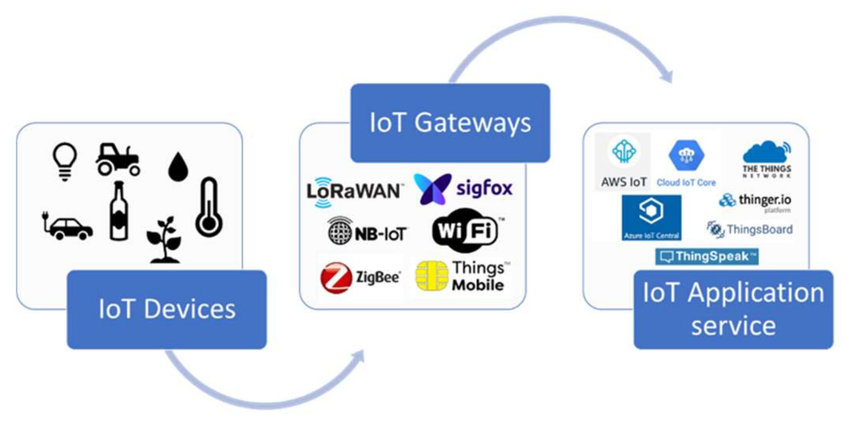
\includegraphics[width=0.9\textwidth]{img/teoria/iot.png}
    \caption{Infraestructura de componentes de un sistema \acrshort{iot} \cite{iotscheme}}
    \label{fig:iot}
\end{figure}

\subsection{IoE}
\label{sec:ioe}

Considerando el contexto energético en el que se engloba este \gls{tfm} y entrando con más detalle en el marco de las tecnologías \gls{iot}, es preciso destacar dentro de las mismas la subcategoría denominada como el Internet de la Energía (del ingles \gls{ioe}) \cite{ioe}. Como concepto, el \gls{ioe} comprende todo el paradigma de operación de los elementos que constituyen una red energética. Es decir, lleva a cabo la integración de todos los dispositivos, sensores o equipos informáticos en una misma estructura, la cual está basada en internet para poder monitorizar y controlar remotamente cada punto de la red.

\vspace{3mm}

Se puede expresar que, con la implementación de tecnologías basadas en \gls{ioe}, se buscan objetivos muy similares a las \gls{sg}s. No obstante, el \gls{ioe} va más allá y supone un control y una gestión de la red a mayor escala. En otros términos, no solo se constituye por los elementos de la propia infraestructura eléctrica, sino que también permite una gestión energética a nivel interna de los hogares, mediante la inclusión de electrodomésticos y otros dispositivos electrónicos.



%ver tfg -->
\subsection{Redes LLN}


\subsubsection{RPL}


% %%%%%%%%%%%%%%%%%%%%%%%%%%%%%%%%%%%%%%%%%%%%%%%%%%%%%%%%%%%%%%%%%%%%%%%%%%%%%%%%%%%%%%%%%%%%%%%%%%%%%
%%%%%%%%%%%%%%%%%%%%%%%%%%%%%%%%%%%%%%%%%%%%%%%%%%%%%%%%%%%%%%%%%%
\section{DEN2NE}
\label{sec:den2ne}

funcionamiento del algoritmo

\cite{den2ne}
\cite{gitden2ne}





% %%%%%%%%%%%%%%%%%%%%%%%%%%%%%%%%%%%%%%%%%%%%%%%%%%%%%%%%%%%%%%%%%%%%%%%%%%%%%%%%%%%%%%%%%%%%%%%%%%%%%
%%%%%%%%%%%%%%%%%%%%%%%%%%%%%%%%%%%%%%%%%%%%%%%%%%%%%%%%%%%%%%%%%%
\section{Big Data}
\label{sec:bigdata}


El \textit{Big Data} \cite{stab} se puede definir como el manejo y el análisis de un conjunto extremadamente grande de datos, los cuales provienen de fuentes diferentes y no correlacionadas. Debido a su complejidad y volumen, no pueden ser procesados con software o herramientas tradicionales de gestión de bases de datos y se requieren soluciones tecnológicas más avanzadas. El concepto de \textit{Big Data} se basa en tres componentes principales, denominadas como las 5 Vs \cite{5vs} \cite{5vs2}:

\begin{itemize}
    \item Variedad: Hace referencia a la heterogeneidad de la información. Existen distintos tipos de datos a procesar de diferentes fuentes, formas y resoluciones. Se puede simplificar su gestión si estos son estructurados (en forma de tablas de bases de datos) o dificultar, si estos no tienen una estructura definida (en formato de texto o imagen). También, pueden ser semiestructurados (en formato JSON o XML).
    \item Velocidad: Es un parámetro crítico, ya que algunos entornos requieren de una toma de decisiones a tiempo real y los datos deben de ser generados, procesados y analizados rápidamente. 
    \item Volumen: Es imprescindible tener la capacidad de gestionar una gran cantidad de datos (en el orden de los TB) que además, es creciente en el tiempo. El almacenamiento y la minería de datos deben de ser eficientes para manejarlos de forma correcta 
    \item Veracidad: Mide la calidad y confiabilidad de la información que se adquiere. Se comprueba su autenticidad e integridad para asegurar que proviene de una fuente legítima, por lo que se deben aplicar mecanismos de seguridad como la encriptación o herramientas de detección y mitigación de ataques a la red (ver Sección \ref{sec:seg}). También, se verifica que la información no contenga errores y que sea lo más precisa posible.
    \item Valor: La masividad de datos introduce mucho ruido y confusión en la información y debe de seleccionarse solamente aquella de utilidad, aplicando minería de datos y procesamiento adicional.
\end{itemize}

\vspace{1mm}

Durante los últimos años el \textit{Big Data} se ha adoptado en multitud de sectores y campos como en las telecomunicaciones, las finanzas, el comercio, la medicina, el transporte o la investigación científica. Como se ha expuesto en los apartados anteriores (ver Sección \ref{sec:smartgrids} y, en particular, \ref{sec:consumo}) y, poniendo enfoque en los objetivos de este \gls{tfm} (ver Sección \ref{sec:obj}), el \textit{Big Data} tiene un gran potencial en el ámbito de las \gls{sg}s.

\vspace{3mm}

En este contexto, la efectividad del empleo de la información reside en la búsqueda de la correlación entre los datos adquiridos de la red eléctrica y el resto de características que pueden influir en los mismos, como son el comportamiento de los usuarios finales, las condiciones de estabilidad, la disponibilidad de recursos, el estado de las cargas o las condiciones climáticas en un determinado instante temporal. La coordinación de las mediciones que se realizan en la red junto con la información que se dispone del entorno es crucial para la monitorización, el control y la operativa llevada a cabo dentro de la \gls{sg}.~\cite{stab} 

\vspace{3mm}

En otros términos, un análisis efectivo del \textit{Big Data} conducirá a una buena toma de decisiones en el sistema y, en consecuencia, a su optimización. Este análisis se constituye del empleo de herramientas dedicadas al procesamiento distribuido, el almacenamiento en la nube, la minería de datos y a técnicas y algoritmos de aprendizaje automático (\gls{ml}). 

\vspace{3mm}

\subsection{Computación en nube}

En la Figura \ref{fig:bigdata2} se representa la infraestructura de procesos dedicados al \textit{Big Data} en un ámbito de \gls{sg}s. Como se puede visualizar, se compone de tres capas operativas: la superior está enfocada al almacenamiento y computación de datos, la intermedia, a la gestión, compartición e integración de datos de diferentes aplicaciones o fuentes y la inferior, a todos los procesos y técnicas que se encargan del procesamiento, minería, clusterización y clasificación final. \cite{stab} 

\begin{figure}[h!]
  \centering
  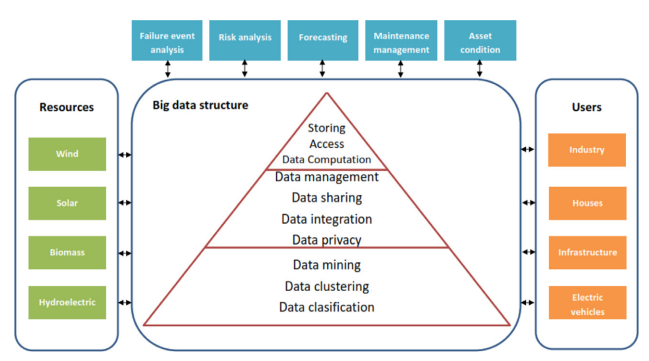
\includegraphics[width=0.9\textwidth]{img/teoria/bigdata2.png}
  \caption{Infraestructura de \textit{Big Data} enfocada al ámbito de las \acrshort{sg}s \cite{stab}}
  \label{fig:bigdata2}
\end{figure}

Para implementar esta infraestructura, es preciso hacer uso de un entorno de computación en nube. Dentro de este contexto, las grandes tecnológicas como Google, Amazon y Microsoft han puesto sus esfuerzos en los últimos años en desarrollar y optimizar sus propios entornos de nube con el fin de integrar toda la gestión y análisis del \textit{Big Data} en una plataforma. A modo de aportar una mayor comprensión de su funcionamiento, se representa en la Figura \ref{fig:bigdata} un esquema de los servicios de nube disponibles.

\begin{figure}[h!]
  \centering
  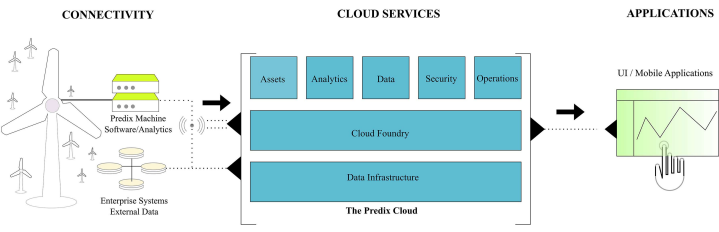
\includegraphics[width=1\textwidth]{img/teoria/bigdata.png}
  \caption{Plataforma de análisis de \textit{Big Data} en el entorno de \acrshort{sg}s \cite{bigdata}}
  \label{fig:bigdata}
\end{figure}

\vspace{3mm}

La computación en la nube se basa en el concepto de virtualización, el cual se puede definir como la tecnología que permite la creación de diferentes entornos virtuales aislados a partir de los recursos hardware disponibles y con independencia de este. Los proveedores de servicios emplean la virtualización para crear múltiples \gls{vm} y ofrecer recursos, como pueden ser el almacenamiento, la potencia de procesamiento o las aplicaciones de la nube, como diferentes servicios virtualizados. Esto aporta las siguientes ventajas a la computación en nube \cite{bigdata} \cite{virt}:

\begin{itemize}
  \item Escalabilidad: Se pueden aumentar o reducir recursos de la nube según las necesidades en cada instante temporal. Los usuarios consiguen un autoprovisionamiento de los recursos, ya que pueden desplegar instancias virtuales cuando lo deseen de forma manual o automática.
  \item Flexibilidad: Se ofrecen muchas posibilidades de configuración de los servicios de la nube.
  \item Interoperabilidad: Se emplean Interfaces de Programación de Aplicaciones (del ingles \gls{api}) para integrar plataformas y aplicaciones heterogéneas. El objetivo es soportar la comunicación entre las mismas y que se produzca una interpretación de los datos de forma correcta. Por ello, también se estandarizan los protocolos para que sean comunes. 
  \item Seguridad: Las plataformas de servicios de nube ofrecen un gran nivel de seguridad e implementan medidas como la encriptación de los datos y restricción de acceso o de permisos. Además, el aislamiento de los recursos y de las aplicaciones en diferentes \gls{vm} permite coonfigurar e implementar diferentes políticas de seguridad según las necesidades.
  \item Ahorro de costes: Se implementa un modelo de pago por uso en función de los recursos que se han consumido y se evita la inversión inicial necesaria para la instalación de una infraestructura física, además de su mantenimiento en el tiempo (CAPEX y OPEX).
  \item Disponibilidad: Se garantiza el acceso a los servicios y la confiabilidad de los mismos. Para ello, implementa técnicas de redundancia y aporta una buena toleracia a fallos.
\end{itemize}









\vspace{3mm}









%hablar de mineria de datos -> 3.2 datos inciertos (vacios y tal), 3.4 y 3.5



%stab

%Over the past few years, big data tools have been adopted by
% many major companies in the power industry such as IBM, Siemens,
% General Electric and Oracle (Arenas-Martinez et al., 2010). According to Li et al. (2012), about 85% of the processing tasks of big
% data can be delayed by a day. Hence, even if the energy output is
% time-varying and intermittent, it can be leveraged for processing the
% delayed datasets. Every day, more Terabytes of data emerge at the
% energy data center. Hence, it has become crucial to adopt big data
% technology to extract information from the multiple and diverse data
% sources through novel data centers (Liu et al., 2012). Through BDA, it
% would be possible to understand the behavior of energy consumption,
% which would help to improve energy efficiency and also promote the
% concepts of sustainability (Koseleva & Ropaite, 2017; Marmaras et al.,
% 2017; Mostafa & Negm, 2018).





%%bigdata

% 2.2 Industry perspective
% Even though the information technology related companies have
% achieved substantial success in the field of big data analytics,
% electrical industries are at the beginning stage to deploy big data. A
% few industries including Siemens, GE, ABB, OSI-Soft, and so on
% are developing big data platform and analytics for power grids. An
% account of a few commercially available platforms is provided here
% as a sample only and by no means is intended to be exhaustive.
% Siemens has developed a big data platform, called EnergyIP
% Analytics, which adds big data to smart grid application and
% provides insights on the management of big data for providing
% various grid services to electric utilities and grid operators [40].
% Siemens is currently integrating utility operations and data
% management technologies that could potentially be tapped for grid
% data analytics. This grid analytics platform can allow utilities to
% utilise big data for multiple functionalities, including home energy
% management, grid energy management, and predictive/corrective
% controls [40]. EnergyIP Analytics has already been used by more
% than 50 utilities with a total of 28 million installed smart devices
% [41].
% Similarly, GE has developed an industrial IoT platform, called
% PREDIX, to consolidate data from existing grid management
% systems, smart meters, and grid sensors [42]. In addition, Grid IQ
% Insight, a cloud-based big data analytics architecture, which utilises
% PREDIX platform, is developed to integrate big data analytics to
% grid applications [43]. Native data collected from Grid IQ Insight
% are stored in Data Lake that could be tapped for several grid
% applications [44]. In fact, these initiatives and developments
% support multiple grid applications ranging from real-time grid
% monitoring, distribution automation, home energy management,
% and ancillary services. As illustrated in Fig. 7, a concept of edgcomputing, whereby computational intelligence is connected at theedge of the data source, has been introduced by GE in its Grid IQInsight.
%ABB is integrating cloud computing and big data analytics
% intended for future power grid applications. ABB has developed an
% intelligent big data platform, called ABB Asset Health Center,
% which provides solutions for processing big data for smart grid
% applications [45]. In fact, ABB's Asset Health Center embeds
% equipment monitoring and systems expertise to establish end-toend asset management, business processes for reducing costs,
% minimising risks, improving reliability, and optimising operations
% across the electric utility [45]. In addition, OSI-Soft PI system,
% which is one of the most widely deployed database and analytics
% system, has been contributing to unveil the power of big data
% analytics to electric utilities. Smart asset management platform has
% introduced by OSI-Soft for the purpose of real-time monitoring of
% asset health [46].
% The aforementioned industries are offering utilities a way to
% gain a core understanding of what is the state of grid devices, and
% developing a launching pad for smart grid big data analytics
% applications over time. The next step for the industries is to
% effectively integrate prognosis and diagnosis into big data analytics
% framework so as to facilitate utilities to provide situational
% awareness, informed predictive decisions, condition monitoring,
% health management of critical grid infrastructure, and supporting
% grid functionalities.





















%ver (teoria)%20Smart-grid-based-big-data-analytics-using-machine-learning-and-artificial-intelligence-a-survey.pdf





% %%%%%%%%%%%%%%%%%%%%%%%%%%%%%%%%%%%%%%%%%%%%%%%%%%%%%%%%%%%%%%%%%%%%%%%%%%%%%%%%%%%%%%%%%%%%%%%%%%%%%
%%%%%%%%%%%%%%%%%%%%%%%%%%%%%%%%%%%%%%%%%%%%%%%%%%%%%%%%%%%%%%%%%%
\section{Inteligencia Artificial}
\label{sec:iateoria}

La inteligencia artificial (\gls{ia}) se constituye como la disciplina de diseño y creación de sistemas de software o hardware de imitación de la inteligencia humana para la realización de tareas. Generalmente, estos sistemas obtienen la capacidad de aprendizaje, razonamiento, planificación y toma de decisiones a partir del entrenamiento basado en grandes cantidades de información. En otros términos, adquieren e interpretan datos del entorno o de un contexto específico y, teniendo en cuenta un objetivo determinado, procesan la información contenida para decidir la siguiente acción a realizar. Adicionalmente, son capaces de adaptar su comportamiento ante el análisis o detección de cambios en el entorno. \cite{iagov} \cite{iaazure}

\vspace{3mm}

La \gls{ia} se postula como una de las tecnologías más revolucionarias y transformadoras de la actualidad y del futuro cercano por su potencial de aplicación en numerosos ámbitos. No obstante, el origen del término se remonta al año 1956, cuando el científico John McCarthy introdujo la idea de crear máquinas inteligentes tomando como base las teorías de computación de los matemáticos Norbert Wiener y John von Neumann en los años 40.~\cite{iagov}

\vspace{3mm}

En la última década, el impulso de la \gls{ia} y los grandes avances que se han producido en este campo vienen dados principalmente por el aumento de las capacidades de los equipos informáticos y el acceso a grandes cantidades de recursos computacionales en las herramientas especializadas e infraestructuras de nube. En otros términos, se posibilita un almacenamiento masivo de datos y, en consecuencia, mejoras significativas en el desarrollo de algoritmos y técnicas, que cada vez se vuelven más complejas y precisas. Además, cabe destacar la contribución que han supuesto las tecnologías \gls{iot} (ver Sección \ref{sec:iot}) en la generación de grandes volúmenes de datos y, por tanto, en el avance de la \gls{ia} al proporcionar información de valor con la que entrenar estos algoritmos.

\vspace{3mm}

Entrando en estas técnicas, se establecen dos divisiones dentro del campo de la \gls{ia} en función de la naturaleza del aprendizaje: el automático (\acrfull{ml}) y el profundo (\acrfull{dl}). En las siguientes Secciones (ver Secciones \ref{sec:ml} y \ref{sec:dl}) se expondrán las características que presentan cada una de estas ramas, además de entrar en profundidad en el funcionamiento de los modelos que se emplearán en el desarrollo de este \gls{tfm}.

\subsection{Machine Learning (\acrshort{ml})}
\label{sec:ml}

La rama de aprendizaje automático (\acrfull{ml}) se enfoca en el desarrollo de modelos que sean capaces de aprender y tomar decisiones en base a la introducción de datos. Durante el proceso se realizan observaciones a la información existente y, en función de la técnica a emplear, se aplican algoritmos estadísticos para identificar patrones en los datos. Por lo tanto, mediante un entrenamiento progresivo en el tiempo, un modelo de \gls{ml} puede llegar a realizar predicciones sobre datos futuros sin la intervención humana y con una alta precisión. Como se representa en la Figura \ref{fig:ml}, las técnicas de \gls{ml} pueden pertenecer a tres categorías diferentes en función del enfoque de la información y de los objetivos que se pretenden conseguir con su aplicación: \cite{mlcat} \cite{iageeks} \cite{mltlf}

\vspace{3mm}

\begin{figure}[h!]
    \centering
    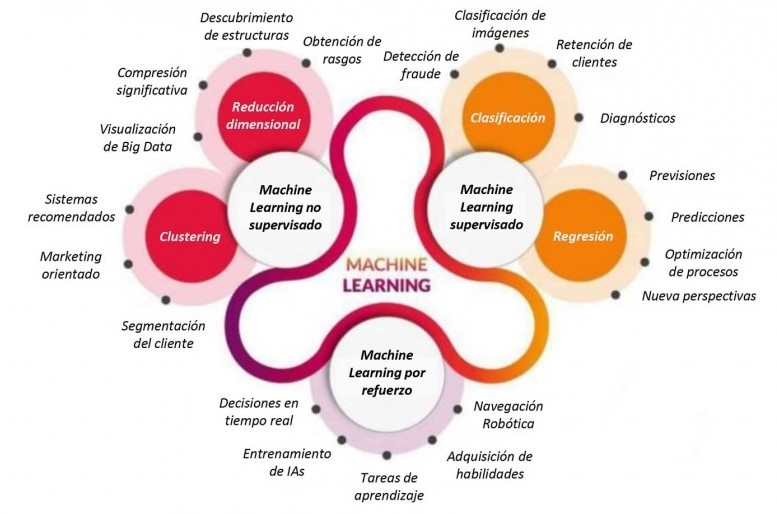
\includegraphics[width=1\textwidth]{img/teoria/ml.jpeg}
    \caption{Categorías de \acrshort{ml} \cite{metal}}
    \label{fig:ml}
\end{figure}

\begin{itemize}
    \item Aprendizaje no supervisado: Se parte de datos sin etiquetar para el entrenamiento de los modelos. Es decir, se parte del conocimiento de unos datos de entrada, pero no de la salida, por lo que el objetivo de los modelos no supervisados se basa en explorar posibles patrones en los datos mediante \textit{clustering}.
    \item Aprendizaje supervisado: Se manejan conjuntos de datos con un conocimiento de las posibles salidas, las cuales se proporcionan en forma de etiquetas o de valores numéricos. Las técnicas de aprendizaje supervisado buscan una función óptima que consiga, dadas unas determinadas variables o características de entrada, predecir la salida con cierta precisión. Son aplicables a dos tipos de problemas: de regresión, si a partir de las variables de entrada se desea predecir un valor numérico continuo a la salida, o de clasificación, si se predefinen diferentes clases y se asignan las variables de entrada a una de ellas. 
    \item Aprendizaje por refuerzo: Las técnicas englobadas en este tipo aprenden por prueba y error, por lo que su entrenamiento a lo largo del tiempo y la experiencia permiten optimizar los resultados sin la necesidad de disponer de un gran volumen de datos.
\end{itemize}

Una vez expuestas las diferentes categorías donde se engloban las técnicas de \gls{ml}, es preciso indicar que se va a centrar el estudio en el \textbf{aprendizaje supervisado} y, en particular, en la resolución de problemas de \textbf{clasificación binaria}. El motivo principal viene dado porque el objetivo que se persigue con la realización de este \gls{tfm} se basa en el desarrollo de modelos que permitan detectar y predecir posibles errores que se pueden producir en una \gls{sg} durante el proceso de distribución energética. 

\vspace{3mm}

Como se detallará más adelante en la Sección \ref{sec:cambiosden2ne}, se creará un conjunto de datos etiquetados en función de la existencia de error o no para entrenar los modelos. Teniendo en cuenta esto, a continuación, se incluyen dos Secciones (ver Secciones \ref{sec:mlsvm} y \ref{sec:mlrf}) para presentar el funcionamiento de las dos técnicas de \gls{ml} que se desarrollarán posteriormente.

\subsubsection{Random Forest (\acrshort{rf})}
\label{sec:mlrf}

El modelo de Bosques Aleatorios (del inglés \acrfull{rf}) está fundamentado en la aplicación de un conjunto de árboles de decisión. Cada uno de estos árboles se definen como estimadores y crecen mediante un proceso de entrenamiento sobre un subconjunto de datos extraído de forma aleatoria del conjunto completo. A la salida del esquema de estimadores se obtiene una predicción final basada en la votación mayoritaria de los árboles. No obstante, es un método que se puede emplear también en problemas de regresión y, en este caso, se proporcionaría un valor numérico promedio, calculado a partir de todas las salidas. En la Figura \ref{fig:rf}, se representa de forma gráfica el diagrama de flujo que expone el funcionamiento del modelo. \cite{rfmedium}

\vspace{3mm}

El proceso de construcción de los árboles de decisión se constituye por operaciones de división que van formando nodos y ramificaciones de forma iterativa. El objetivo es lograr la mayor ganancia de información posible a través de la valoración de la importancia que presentan cada una de las características del conjunto de datos. En otros términos, en cada nodo \textit{m} del árbol se cuantifica la ganancia de información que presenta cada característica y, después, se selecciona la que tenga el mayor valor (\textit{j}). Se aplica una división de los datos existentes en dos subconjuntos homogéneos de menor tamaño: \cite{rfmedium2}

\begin{equation}
    \begin{aligned}
        \theta &= (j, t_m) \\
        Q_m^{\text{left}}(\theta) &= \{(x, y) \mid x_j \leq t_m\} \\
        Q_m^{\text{right}}(\theta) &= Q_m \setminus Q_m^{\text{left}}(\theta)
    \end{aligned}
\end{equation}
    

Donde:
\begin{itemize}
    \renewcommand{\labelitemi}{}
    \item \( \theta \) es la operación de división en un nodo \textit{m}.
    \item \( j\) es la característica seleccionada.
    \item \( t_m\) es el nivel de partición de los datos.
    \item \( Q_m^{left}\) es el subconjunto de datos en la ramificación izquierda.
    \item \( Q_m^{right}\) es el subconjunto de datos en la ramificación derecha.
\end{itemize}

\vspace{3mm}

\begin{figure}[h!]
    \centering
    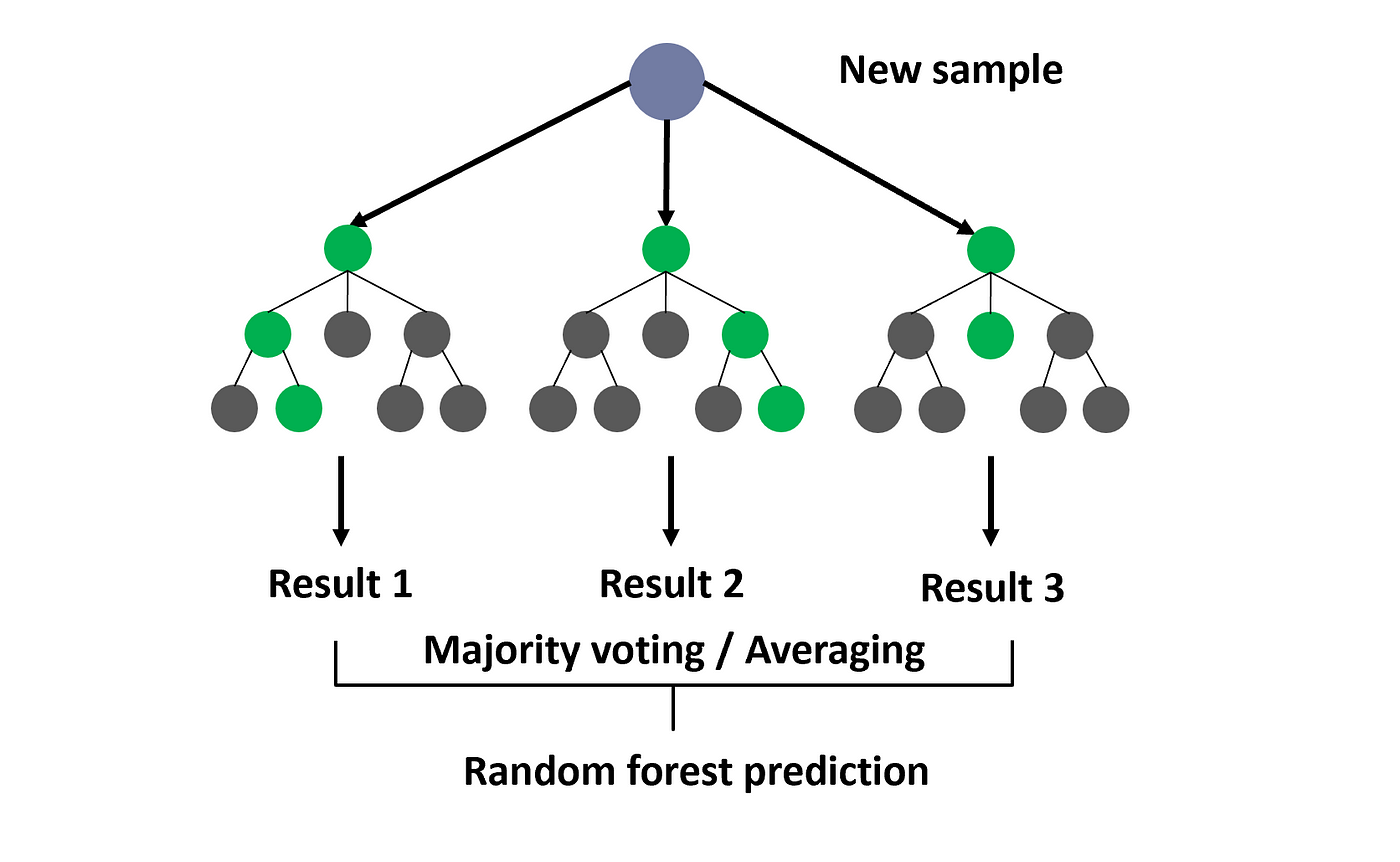
\includegraphics[width=0.95\textwidth]{img/teoria/rf.png}
    \caption{Modelo \acrshort{rf} \cite{rfmedium}}
    \label{fig:rf}
\end{figure}

\vspace{3mm}

Este proceso se va repitiendo en todos los nodos hasta llegar al final del árbol y, en cuanto al cálculo de la ganancia de información, es preciso introducir el concepto de impureza. Este se define como el procedimiento de evaluación de la calidad de las divisiones que se producen en los nodos. En otros términos, se puede expresar que indica el nivel de ruido que hay en los datos de los subconjuntos creados mediante una función de impureza \textit{H()}:

\vspace{3mm}

\begin{equation}
    \begin{aligned}
        G(Q_m, \theta) = \frac{n_m^{left}}{n_m} H(Q_m^{left}(\theta)) + \frac{n_m^{right}}{n_m} H(Q_m^{right}(\theta))
    \end{aligned}
\end{equation}

\vspace{3mm}

Tomando esto en consideración, se pueden emplear dos funciones o métodos de medición de la impureza:~\cite{rfmedium2} \cite{scikitrf}

\begin{itemize}
    \item Entropía: Su objetivo está orientado a establecer divisiones de los datos de forma que la entropía en los nodos inferiores o hijos sea menor que la del nodo superior o padre. Para ello, se aplica la teoría de la entropía de Shannon \cite{rfmedium2} para escoger las características que minimicen la entropía y, en consecuencia, la incertidumbre y la función de pérdidas. De forma contraria, en un nodo se obtiene una entropía máxima cuando las clases están representadas homogéneamente en el conjunto de datos.
    
    \begin{equation}
        \begin{aligned}
            H(Q_m) = - \sum_k p_{mk} \log(p_{mk})
        \end{aligned}
    \end{equation}
    
    \item Gini: La impureza es definida a partir del cálculo de la probabilidad de una característica determinada que es clasificada erróneamente cuando se selecciona aleatoriamente. Un índice Gini nulo expresa una clasificación pura donde todos los datos corresponden a una clase específica, en cambio, un índice Gini igual a 1, representa una distribución aleatoria de los datos.
    
    \begin{equation}
        \begin{aligned}
            H(Q_m) = \sum_k p_{mk} (1 - p_{mk})
        \end{aligned}
    \end{equation}
\end{itemize}

Donde:
\begin{itemize}
    \renewcommand{\labelitemi}{}
    \item \(p_{mk}\) es la proporción de datos de entrenamiento que pertenecen a una clase determinada.
    \item \(H(Q_m)\) es la función de impureza.
\end{itemize}


\subsubsection{Support Vector Machines (\acrshort{svm})}
\label{sec:mlsvm}

El modelo de Máquinas de Vector Soporte (del inglés \acrfull{svm}) es una técnica que se emplea tanto en problemas de regresión como de clasificación. Se basa en el concepto del \textit{Maximal Margin Classifier} o \textit{Hard Margin Classifier}, puesto que tiene el fin principal de encontrar el hiperplano óptimo que consiga una máxima separación entre dos clases diferentes dentro de un espacio de características. Esta separación se define como margen y se mide como la distancia perpendicular que existe desde el hiperplano hacia los vectores de soporte, que son las muestras más cercanas a la frontera de separación de clases. En la Figura \ref{fig:svm}, se representa el cálculo del mejor hiperplano entre dos clases de datos. \cite{svmmedium2} \cite{svmciencia}

\vspace{3mm}

Por ello, se puede expresar que los vectores de soporte son los puntos más críticos del plano para asignar una de las clases predefinidas a los nuevos vectores de datos a la entrada. Este proceso de clasificación viene dado por la siguiente expresión: \cite{svmmedium} 

\begin{equation}
    \begin{aligned}
        y_i(\mathbf{w} \cdot \mathbf{x_i} + b) \geq M
    \end{aligned}
\end{equation} 

    Donde:
\begin{itemize}
    \renewcommand{\labelitemi}{}
    \item \(y_i\) es la etiqueta de la clase. 
    \item \(x_i\) es el vector de características.
    \item \(w\) es el vector de pesos o coeficientes del hiperplano.
    \item \(b\) es el sesgo ajustado en el modelo.
    \item \(M\) es el ancho definido para el margen.
\end{itemize}

\vspace{3mm}

\begin{figure}[h!]
    \centering
    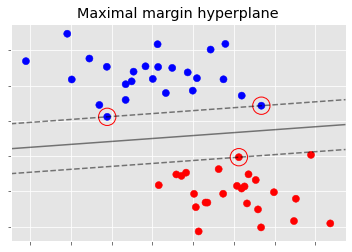
\includegraphics[width=0.65\textwidth]{img/teoria/svm.png}
    \caption{Cuantificación del hiperplano óptimo entre dos clases en el \acrshort{svm} \cite{svmmedium2}}
    \label{fig:svm}
\end{figure}

\vspace{3mm}

No obstante, en la práctica es complicado determinar un hiperplano si no se trata de un problema ideal y basado en datos linearmente separables. Generalmente, en los casos reales si se intenta forzar un máximo margen, se pueden llegar a producir problemas de sobreentrenamiento, ya que nuevos datos pueden suponer grandes variaciones en el hiperplano. En la Figura \ref{fig:svmerror}, se representa la opción alternativa que se lleva a cabo en la mayoría de casos, basada en obtener un margen máximo, permitiendo cierto grado de error (\textit{Soft Margin Classifier}). \cite{matlab} \cite{svmciencia}

\vspace{3mm}

Esto tiene como consecuencia que existan una serie de vectores clasificados de forma errónea en el plano. En este proceso se introduce el concepto de variables de holgura (\textit{slack variables}) a partir de la siguiente expresión:

\begin{equation}
    \begin{aligned}
        \xi_i = \max(0, 1 - y_i (\mathbf{w} \cdot \mathbf{x}_i + b))
    \end{aligned}
\end{equation} 

\vspace{3mm}

\begin{figure}[h!]
    \centering
    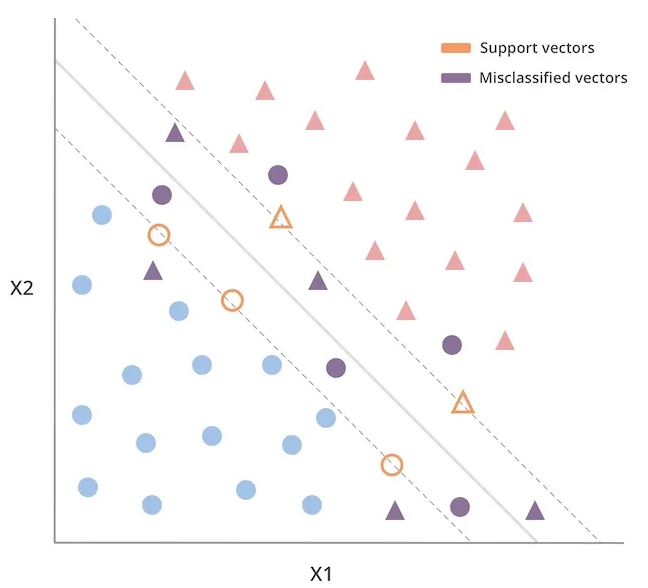
\includegraphics[width=0.65\textwidth]{img/teoria/svm2.png}
    \caption{Representación de vectores clasificados erróneamente dentro de los márgenes establecidos en el \acrshort{svm} \cite{svmmedium}}
    \label{fig:svmerror}
\end{figure}

\vspace{3mm}

Estas variables determinan si un vector está correctamente clasificado o si se encuentra en una zona errónea del margen o del hiperplano, respectivamente. En el caso de posición incorrecta, el valor de la variable define la distancia al margen o el error cometido:

\begin{equation}
    \begin{aligned}
        \xi_i = 0 & \text{ si } 1 - y_i (\mathbf{w} \cdot \mathbf{x}_i + b) \leq 0 \\
        0 \text{<} \xi_i \text{<} 1 & \text{ si } 0 < 1 - y_i (\mathbf{w} \cdot \mathbf{x}_i + b) \leq 1 \\
        \xi_i \text{>} 1 & \text{ si } 1 - y_i (\mathbf{w} \cdot \mathbf{x}_i + b) > 1 \\
    \end{aligned}
\end{equation} 

\pagebreak

El sumatorio de todas las variables de holgura que existen en el plano vienen incluidas en el objetivo de la función de pérdida del modelo para que el error de clasificación sea mínimo, a la vez que el margen es máximo. Como es preciso encontrar un cierto equilibrio entre ambos, el \gls{svm} se determina como una técnica de optimización convexa que se fundamenta en el hiperparámetro \textit{C}. En la Figura \ref{fig:parametroc}, se representa de forma gráfica cómo su valor establece el control de forma inversamente proporcional de la cantidad de muestras clasificadas erróneamente, por lo que se define como el parámetro de regularización del modelo. Es decir, cuanto más alto sea su valor, menores violaciones del margen y del hiperplano serán permitidas y más se enfocará el modelo en un \textit{Maximal Margin Classifier}.~\cite{svmciencia}

\vspace{3mm}

\begin{figure}[h!]
    \centering
    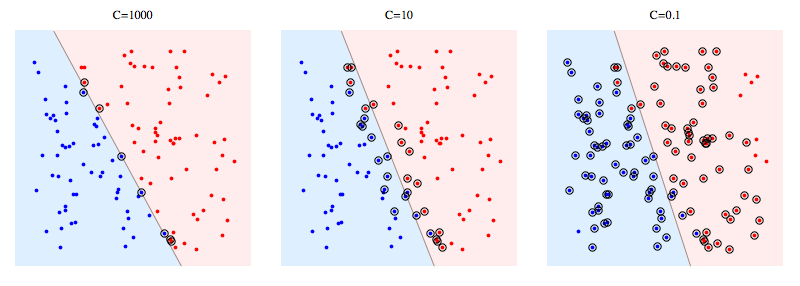
\includegraphics[width=1\textwidth]{img/teoria/parametroc.png}
    \caption{Configuración del parámetro de regularización \textit{C} \cite{velocity}}
    \label{fig:parametroc}
\end{figure}

\vspace{3mm}

Además de permitir cierto grado de error, como se ha expuesto anteriormente, para enfrentar problemas con datos no linearmente separables, es imprescindible incrementar las dimensiones del espacio original de características. En este caso, se introduce el concepto de kernel como función para obtener un nuevo espacio dimensional diferente al original donde exista una mayor probabilidad de que los datos sí sean linearmente separables. La aplicación de los diferentes tipos de kernels que permiten las \gls{svm} se caracteriza a partir de las expresiones expuestas a continuación:~\cite{svmciencia}~\cite{velocity}

\begin{equation}
    \begin{aligned}
        \text{Kernel lineal: } K(\mathbf{x}_i, \mathbf{x}_j) = \mathbf{x}_i \cdot \mathbf{x}_j \\
        \text{Kernel polinómico: } K(\mathbf{x}_i, \mathbf{x}_j) = (\gamma \mathbf{x}_i \cdot \mathbf{x}_j + r)^d \\
        \text{Kernel radial o gaussiano: } K(\mathbf{x}_i, \mathbf{x}_j) = \exp \left( -\gamma \| \mathbf{x}_i - \mathbf{x}_j \|^2 \right) \\
        \text{Kernel sigmoid: } K(\mathbf{x}_i, \mathbf{x}_j) = \tanh(\gamma \mathbf{x}_i \cdot \mathbf{x}_j + r)
    \end{aligned}
\end{equation}


\vspace{3mm}

Para obtener una mayor compresión, se representa de forma adicional la Figura \ref{fig:rbf}. En la misma se puede apreciar gráficamente cómo se produce la transformación dimensional de las características, especificando para el caso del kernel gaussiano o \gls{rbf}.

\vspace{3mm}

\begin{figure}[H]
    \centering
    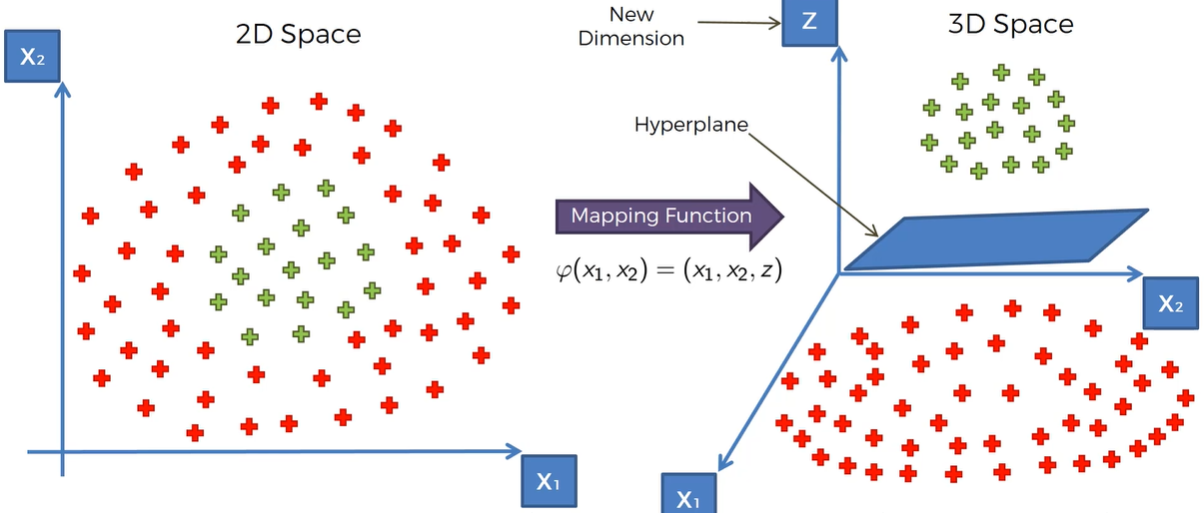
\includegraphics[width=0.9\textwidth]{img/teoria/rbf.png}
    \caption{Aplicación del kernel \acrshort{rbf} \cite{rbf}}
    \label{fig:rbf}
\end{figure}

\subsection{Deep Learning (\acrshort{dl})}
\label{sec:dl}

El campo del aprendizaje profundo (\acrfull{dl}) se enfoca principalmente en la creación de redes neuronales que imiten el comportamiento y la estructura lógica que tiene el cerebro humano para buscar patrones en los datos. A diferencia de las técnicas de \gls{ml}, el \gls{dl} se vuelve mucho más eficiente en el análisis de grandes volúmenes de datos, puesto que generalmente el \gls{ml} presenta ciertas limitaciones en este aspecto. \cite{metal} 

\vspace{3mm}

De la misma forma, el \gls{dl} presenta un mejor funcionamiento en la identificación de patrones cuando se manejan características complejas o un gran número de ellas, aportando resultados con una mayor precisión que el \gls{ml}. Es por ello que las técnicas de \gls{dl} cobran una gran importancia en entornos donde los datos no son estructurados, como se produce en el caso de las imágenes, texto y audio. En este caso, se pueden introducir en aplicaciones de reconocimiento de voz, procesado de lenguaje natural (del inglés \gls{nlp}) o visión artificial para la detección de objetos y clasificación de imágenes. \cite{iageeks}

\vspace{3mm}

De la misma forma, a nivel estructural, las diferencias entre las técnicas de \gls{ml} y las de \gls{dl} radican principalmente en el tratamiento de las características o variables de los datos. En el caso de emplear \gls{ml}, si se manejan conjuntos con un gran número de características, sería necesario introducir un paso previo de diseño y selección de las más relevantes. Esto, como se puede apreciar en la Figura \ref{fig:features}, no ocurre en el desarrollo de un modelo de \gls{dl}, ya que el tratamiento se produce internamente dentro de la red reuronal. \cite{valohai}

\vspace{3mm}

Una vez presentada la rama de aprendizaje profundo, se introduce una Sección dedicada a la exposición del modelo de \gls{dl} que se desarrollará para lograr los objetivos de este \gls{tfm} (ver Sección \ref{sec:dlann}). 

\vspace{3mm}

\begin{figure}[h!]
    \centering
    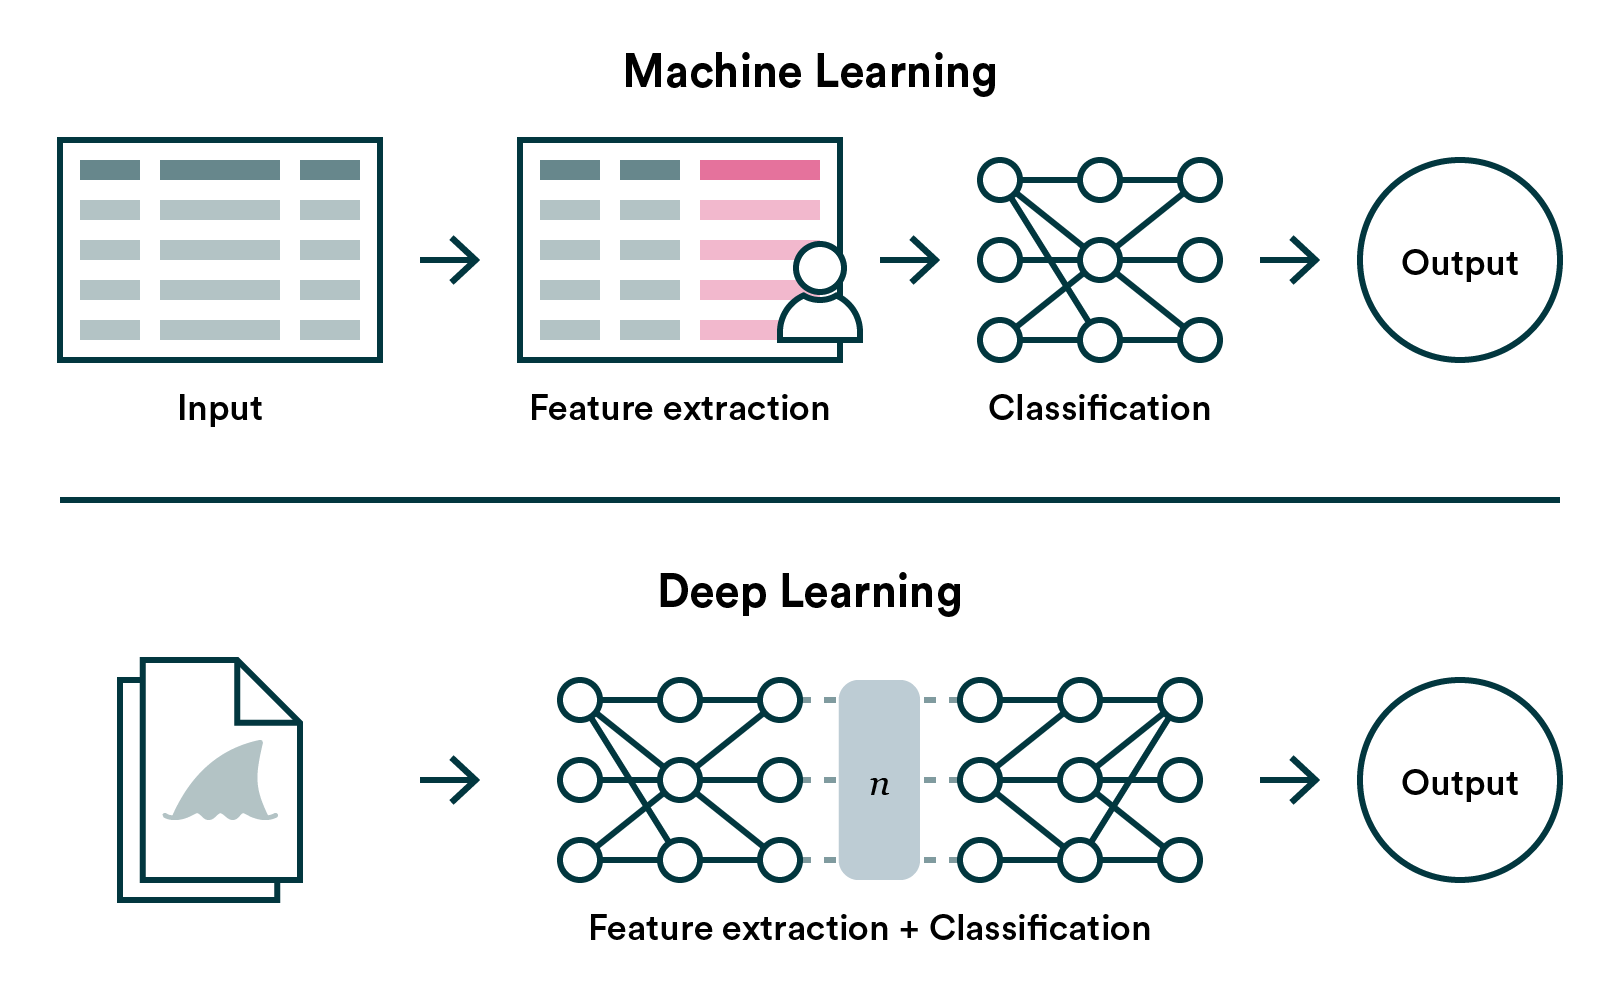
\includegraphics[width=0.8\textwidth]{img/teoria/mlvsdl.png}
    \caption{Diferencias estructurales entre el \acrshort{ml} y el \acrshort{dl} \cite{valohai}}
    \label{fig:features}
\end{figure}

\subsubsection{Red Neuronal Artificial (\acrshort{ann}) y Perceptrón Multicapa (\acrshort{mlp})}
\label{sec:dlann}

Las redes neuronales artificiales (\gls{ann}) y, en particular, los perceptrones multicapa (del inglés \gls{mlp}), se construyen a partir de distintas capas de nodos y conexiones que replican la estructura neuronal que tiene el cerebro humano. Como se representa en la Figura \ref{fig:ann}, se define una capa de entrada (\textit{input layer}), una o múltiples capas ocultas (\textit{hidden layer}) y una capa de salida (\textit{output layer}). El entrenamiento de la arquitectura de neuronas viene dado por las conexiones que se van estableciendo entre los nodos de las capas y los pesos y los valores de umbral que se van especificando durante el proceso. \cite{ibmann}

\vspace{3mm}

En otros términos, se toma cada nodo como una aplicación del modelo de regresión lineal, donde se parte de unos datos en la capa de entrada, que son ponderados con unos determinados pesos en cada capa oculta de la siguiente forma:

\begin{equation}
    \begin{aligned}
        z = \mathbf{w}^T \cdot \mathbf{x} + b
    \end{aligned}
\end{equation} 

Donde:
\begin{itemize}
    \renewcommand{\labelitemi}{}
    \item \(z\) es la salida de cada capa oculta. 
    \item \(w\) es el vector de pesos. 
    \item \(b\) es el sesgo.
    \item \(x\) es el vector de entrada
\end{itemize}

\vspace{3mm}

\begin{figure}[h!]
    \centering
    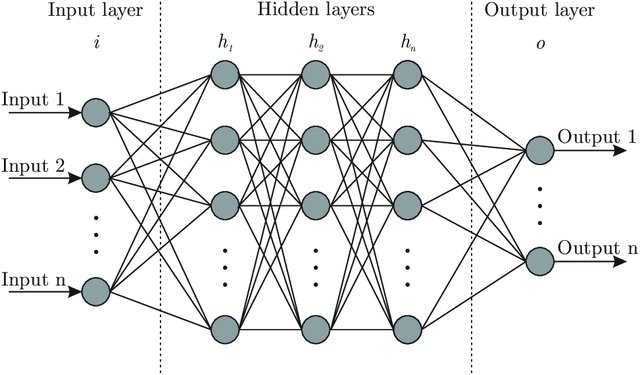
\includegraphics[width=0.75\textwidth]{img/teoria/ann.jpg}
    \caption{Arquitectura de un \acrshort{mlp} \cite{ann}}
    \label{fig:ann}
\end{figure}

\vspace{3mm}

De la misma forma, en cada capa oculta se aplica una función de activación o de umbral, que impone un valor límite a la salida final del nodo en cuestión y, en consecuencia, a la entrada del nodo siguiente al que se encuentre conectado. Las funciones de activación principales que se pueden emplear se representan en la Figura \ref{fig:functions} y vienen dadas por las siguientes expresiones: \cite{factiv} \cite{functions}

\begin{equation}
    \begin{aligned}
        \text{Función Sigmoidal (Logística):} \quad f(x) = \frac{1}{1 + e^{-x}} \\
        \text{Función ReLU (Rectified Linear Unit):} \quad f(x) = \max(0, x) \\
        \text{Función tanh (Tangente Hiperbólica):} \quad f(x) = \tanh(x) \\
        \text{Función Softmax:} \quad \text{softmax}(x_i) = \frac{e^{x_i}}{\sum_{j} e^{x_j}} \\
    \end{aligned}
\end{equation}

\pagebreak

Teniendo todo el procedimiento anterior en cuenta, se puede expresar que, a partir de una serie de características, el objetivo es escoger aquellas que contribuyan a obtener una mayor precisión en la clasificación de datos de entrada futuros, puesto que se van estableciendo las conexiones óptimas entre los nodos de las capas ocultas con un entrenamiento progresivo. Es preciso indicar que el funcionamiento del modelo se basa en una red de propagación hacia delante, lo que supone que se defina un flujo unidireccional, desde la entrada a la salida. 

\vspace{3mm}

\begin{figure}[h!]
    \centering
    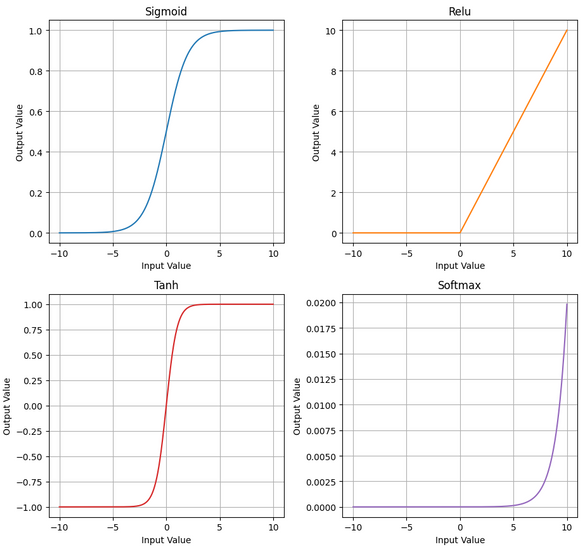
\includegraphics[width=0.75\textwidth]{img/teoria/functions.png}
    \caption{Funciones de activación \cite{functions}}
    \label{fig:functions}
\end{figure}

\vspace{3mm}

No obstante, para ajustar las ponderaciones se aporta una retroalimentación, que depende directamente de la función de coste y de la salida del modelo en cada ejecución o \textit{epoch}. Principalmente, se pueden utilizar dos métodos para minimizar la función de coste: el algoritmo adaptativo \textit{adam} (del inglés \textit{Adaptive Moment Estimation}), que presenta una tasa de aprendizaje adaptativa para cada parámetro, y el gradiente descendiente (del inglés \gls{sgd}), que actualiza los pesos de la red en función del gradiente de la función de pérdida con respecto a los pesos. \cite{ibmann}

\pagebreak

% %%%%%%%%%%%%%%%%%%%%%%%%%%%%%%%%%%%%%%%%%%%%%%%%%%%%%%%%%%%%%%%%%%%%%%%%%%%%%%%%%%%%%%%%%%%%%%%%%%%%%
%%%%%%%%%%%%%%%%%%%%%%%%%%%%%%%%%%%%%%%%%%%%%%%%%%%%%%%%%%%%%%%%%%
\section{Herramientas software}
\label{sec:software}

\subsection{\acrshort{brite}}
\label{sec:brite}

\gls{brite} \cite{brite} se presenta como una plataforma dedicada a la generación de topologías de red. Fue desarrollada en la Universidad de Boston y se caracteriza por su gran flexibilidad, ya que enfoca su arquitectura en el concepto de modelo topológico. Es decir, soporta varios modelos diferentes y cada uno de ellos viene determinado por los parámetros de entrada que se definen. Es por ello que \gls{brite} sigue la siguiente secuencia de acciones para diseñar las topologías:

\vspace{3mm}

\begin{enumerate}
    \item Definición del posicionamiento de los nodos:
    \item Nivel de Interconexión de los nodos y configuración de enlaces:
    \item Asignación de atributos y características de la red y de los dispositivos: Se determina el delay y el ancho de banda de los enlaces.
    \item Especificación del formato de salida: Se indica un formato .brite para todas las topologías generadas.
\end{enumerate}

\vspace{3mm}

En la Sección \ref{sec:ejebrite} se definirán las acciones realizadas con esta herramienta en el caso de este \gls{tfm}. Por otro lado, con el motivo de facilitar el empleo de \gls{brite}, se incluirá una Sección dedicada al proceso de instalación, configuración y ejecución en el Anexo correspondiente a los manuales de usuario (ver Sección \ref{sec:manualbrite}). Se podrá acceder a más información desde el repositorio\footnote{https://github.com/NETSERV-UAH/BRITE} del equipo de investigación NetIS de la \gls{uah}.

\subsubsection{Definición de topologías}
\label{sec:param}

La herramienta \gls{brite} basa el proceso de creación de topologías en la definición de los siguientes parámetros de entrada en un fichero con formato .conf:

\begin{itemize}
    \item \textit{Name}: Modelo de la topología.
    \item \textit{N}: Número de nodos de la topología.  
    \item \textit{HS y LS}: Dimensiones del plano. Respectivamente, hacen referencia a la longitud total del plano cuadrado y al tamaño de los cuadros interiores.
    \item \textit{Node Placement}: Posicionamiento de los nodos. Se puede producir de forma totalmente aleatoria o creando zonas a lo largo del plano con mayor concentración de nodos. 
    \item \textit{Growth Type}: Método de introducción de los nodos en la topología. Se puede realizar este proceso de forma incremental (uno a uno) o de forma aleatoria (todos a la vez). 
    \item \textit{m}: Número de enlaces por nodo o número de nodos vecinos a los que se conectará un nuevo nodo al unirse a la red. \gls{brite} puede crear enlaces unidireccionales o bidireccionales y, respectivamente, la topología generada tendría un grado m o 2m.
    \item \textit{Alpha, Beta}: Parámetros específicos para topologías basadas en el modelo Waxman.
    \item \textit{BWDist, BWMin, BWMax}: Ancho de banda de los enlaces.
\end{itemize}

\subsubsection{Modelos de topologías}
\label{sec:modelostopos}

Como se ha introducido, con \gls{brite} se posibilita el uso de múltiples modelos para crear topologías. En la Figura \ref{fig:brite} se representan todos los que soporta la herramienta. No obstante, este \gls{tfm} se va a enfocar en la generación de topologías a nivel de router, como son los modelos Router Waxman y Router Barabasi-Albert. 

\vspace{3mm}

\begin{figure}[h!]
    \centering
    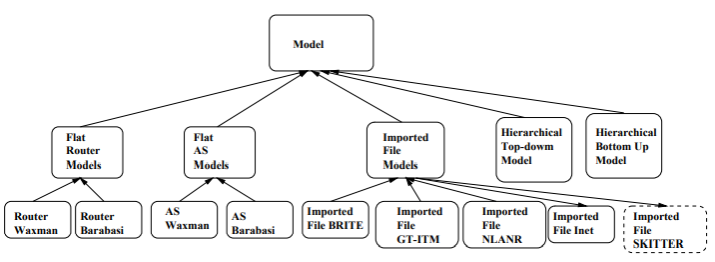
\includegraphics[width=1\textwidth]{img/teoria/brite.PNG}
    \caption{Modelos soportados por \acrshort{brite} \cite{brite}}
    \label{fig:brite}
\end{figure}

\vspace{3mm}

En el caso del Router Waxman, como su nombre indica, emplea un modelo de probabilidad Waxman para establecer la Interconexión de los nodos en la topología \cite{brite_zegura}:

\[P_{\text{Waxman}}(u,v) = \alpha \cdot e^{-\frac{d}{\beta \cdot L}}\]
    
    Donde:
\begin{itemize}
    \renewcommand{\labelitemi}{}
    \item \textit{P(u,v)} es la probabilidad en función de la distancia euclidiana entre un nodo \textit{u} y un nodo \textit{v} de la red.
    \item $\alpha$ es un parámetro específico del modelo que hace referencia a la densidad de enlaces y toma generalmente un valor igual a 0.2.
    \item $\beta$ es un parámetro específico del modelo que hace referencia al ratio enlaces largos/enlaces cortos en la topología y toma generalmente un valor igual a 0.15.
    \item \textit{L} es la máxima distancia entre dos nodos cualesquiera.
\end{itemize}

\vspace{3mm}

Por otro lado, el modelo Router Barabasi-Albert está basado en la generación de topologías con un incremento exponencial del número de nodos a lo largo del tiempo. Además, se permite una conexión preferencial, suponiendo que cuanto mayor grado de conectividad abarque un nodo, mayor será la probabilidad de que este añada nuevos enlaces. Por lo tanto, el plano de la topología comienza con un número de nodos inicial \textit{N0} y se van añadiendo los demás uno a uno. Cada uno de estos nuevos nodos se conectará a \textit{N} nodos ya añadidos a la topología con una probabilidad \cite{brite_zegura}:

\[P_{\text{Barabási-Albert}}(k_i) = \frac{k_i}{\sum_{j}^{}k_j}\]
    
    Donde:
\begin{itemize}
    \renewcommand{\labelitemi}{}
    \item \textit{P(k)} es la probabilidad de conexión del nodo \textit{i} con grado \textit{k}.
    \item $\sum_{j}^{}k_j$ es el sumatorio de los grados de todos los nodos de la topología.
\end{itemize}

\subsubsection{Automatización de la ejecución}
\label{sec:brite_eje}

A modo de facilitar la ejecución de la herramienta \gls{brite} se aporta en el repositorio el fichero de python \textit{generador\_brite.py}, dedicado a la automatización del proceso de creación de un fichero de configuración. Este recibirá los parámetros de entrada que caracterizarán a la topología a generar (ver Sección \ref{sec:param}) y escribirá el nuevo fichero.

\vspace{3mm}

También, se añade el fichero de python \textit{parser.py}, que se encargará de definir la función de transformación del archivo de salida proporcionado por \gls{brite} (en formato .brite) en dos nuevos ficheros: \textit{Nodos.txt} y \textit{Enlaces.txt}. Respectivamente, estos almacenarán las posiciones x e y de los nodos en el plano y la información sobre las distancias y los identificadores de los nodos que se interconectan con cada enlace. Este funcionamiento se muestra de forma gráfica en la Figura \ref{fig:parser}.

\vspace{3mm}

\begin{figure}[H]
    \centering
    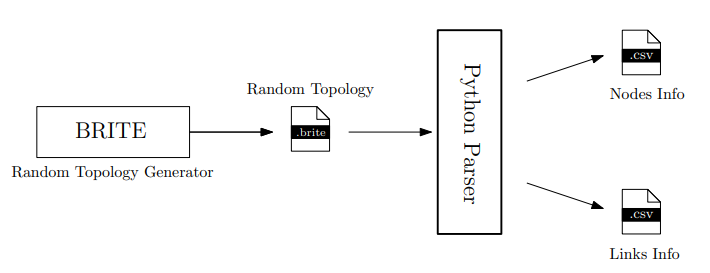
\includegraphics[width=0.7\textwidth]{img/teoria/parser.png}
    \caption{Esquema de funcionamiento de \acrshort{brite} y del \textit{parser} \cite{den2ne}}
    \label{fig:parser}
\end{figure}

\vspace{3mm}

Teniendo en cuenta los ficheros anteriores, se proporciona un script \textit{autogenerador.sh} donde se incluyen todas sus funcionalidades y se automatiza todo el proceso de ejecución de la herramienta. Este script sigue la siguiente secuencia de pasos:

\begin{enumerate}
    \item Define los valores de cada uno de los parámetros de entrada.
    \item Ejecuta el fichero de python \textit{generador\_brite.py} aplicando los parámetros definidos para el modelo Waxman y Barabasi.
    \item Genera 10 topologías diferentes para cada archivo de configuración a partir de 10 ficheros de semillas (\textit{seed\_files}) dados en el repositorio. Esto posibilita la generación de 10 topologías totalmente diferentes para cada escenario de red definido (a partir de unos mismos parámetros de entrada). 
    \item Se aplica un bucle en función del número de semilla:
    \begin{enumerate} 
        \item Crea el directorio para cada escenario y se ejecuta la heramienta \gls{brite} sobre cada uno.
        \item Se ejecuta \textit{parser.py} para obtener a la salida los ficheros \textit{Nodos.txt} y \textit{Enlaces.txt} de cada uno de los escenarios.   
    \end{enumerate} 
\end{enumerate}



